
\documentclass[journal]{IEEEtran}
\usepackage[utf8]{inputenc}
\usepackage{cite}
\usepackage[cmex10]{amsmath}
\interdisplaylinepenalty=2500
\usepackage{algorithmic}
\usepackage{array}
\usepackage{url}
\usepackage{mathtools}
\hyphenation{op-tical net-works semi-conduc-tor method methods}
\usepackage{float}


\ifCLASSOPTIONcompsoc
  \usepackage[caption=false,font=normalsize,labelfont=sf,textfont=sf]{subfig}
\else
  \usepackage[caption=false,font=footnotesize]{subfig}
\fi

\ifCLASSINFOpdf
  \usepackage[pdftex]{graphicx}
  % declare the path(s) where your graphic files are
  % \graphicspath{{../pdf/}{../jpeg/}}
  % and their extensions so you won't have to specify these with
  % every instance of \includegraphics
  \DeclareGraphicsExtensions{.pdf,.jpeg,.jpg,.png}
\else
  % or other class option (dvipsone, dvipdf, if not using dvips). graphicx
  % will default to the driver specified in the system graphics.cfg if no
  % driver is specified.
  \usepackage[dvips]{graphicx}
  % declare the path(s) where your graphic files are
  % \graphicspath{{../eps/}}
  % and their extensions so you won't have to specify these with
  % every instance of \includegraphics
  \DeclareGraphicsExtensions{.eps}
\fi

\floatstyle{ruled}
\newfloat{json}{thp}{lop}
\floatname{program}{Program}

%opening
\title{Hidden Markov Model Baseline for Flexible Assembly System Anomaly Detection - DRAFT}
\author{Tero Keski-Valkama}

\begin{document}

\maketitle
Version: \today

\begin{abstract}

\end{abstract}

\begin{IEEEkeywords}
\end{IEEEkeywords}

\section{Introduction}

Flexible Assembly Systems (FAS) and Flexible Manufacturing Systems (FMS) represent an evolution from specialized mass manufacturing systems. They allow flexibility in manufacturing which enables efficient production of smaller production runs and customization, personalization and quick evolution of manufactured products.

Flexibility brings challenges as it makes fault detection harder, especially in systemic conditions. Even if each separate module of a flexible assembly plant was nominally operating well, there are systemic fault modes and degradations which can cause non-optimal performance of the whole. Novel production plans deployed to the manufacturing system evokes new behaviours and possible problems. As flexible manufacturing generally requires more open integration to external systems for planning and controlling production dynamically, it becomes more susceptible to cyberattacks.

Many of these fault conditions and degradations are such that they cannot be trivially known in advance. Industrial anomaly detection systems are used to detect novel anomalous conditions which might denote faults, degradations or for example cyberattacks. Traditional process mining methods are not well suitable for environments with heterogeneous industrial IoT systems creating logs where process trace events might not be fully correlated with the process ids. These uncorrelated process traces or logs are therefore interlaced so that events are in sequence but originating from separate processes. In general case, automatic process identification might not be even possible in an explicit form.

Machine learning approaches can provide automatic learning of industrial process nominal operation, and those can be used to flag anomalous situations. Machine learning systems require data to train on, and industrial process data is guarded trade secret especially in relation to fault conditions. Real data on manufacturing process faults is nontrivial to get in sufficient amounts and on system level. Hence, simulations for synthetic flexible assembly process are required. In this research, FAS Simulator is used as the data source \cite{keski2017simulator}. Simulated Flexible Assembly System logs are sequences of events recorded during simulated production of a batch of products represented by sequences of categorical symbols.

To compare different machine learning approaches, baselines are needed. We are interested in anomaly detection solutions for uncorrelated process traces, or sequential, interlaced event logs. Existing methods for these include Hidden Markov Model based approaches \cite{gornitz2015hidden}\cite{joshi2005investigating}, denoising autoencoder based approaches \cite{nolle2016unsupervised}, LSTM based approaches \cite{yuan2021recompose}\cite{du2017deeplog}, or even more complex deep neural networks \cite{zhang2019robust}. Some of the traditional approaches such as Alpha algorithm from process mining require correlated process traces, where each event is tagged with the process instance it belongs to, effectively deinterlacing the event logs.

Isolation Forests\cite{liu2008isolation} (IF) and Functional Isolation Forests\cite{staerman2019functional} (FIF) can also be used to evaluate whether an event or a sequence of events is anomalous. Isolation Forests work by growing a random forest by splits of sets of measurements until each measurement is isolated from the others. The length of the route from the root of the measurement will then become a measure of normality, and shorter length paths to measurements imply anomalous measurements. Functional Isolation Forests require defining measurement sequences as functions in a Hilbert space where distances between sequences are well defined. Then a dictionary of examples of sequences can be used as a basis to project each measurement sequence to, and use these base axes for splitting conditions in the random forest.

Isolation Forests are inapplicable to discrete event sequences if the events are categorical, and don't include specific event categories which would imply anomalies without a context. Functional Isolation Forests can be applied to constant-sized windows in variable-length sequences, but as the events in discrete event logs are categorical, they don't have an inner product defined in a sensible fashion so Functional Isolation Forests are inapplicable in their naive forms as well.

Here we present results of applying Hidden Markov Models on FAS Simulator datasets to produce a baseline benchmark for this challenge to compare more sophisticated approaches against.

\section{Setup}

We generated challenge data using FAS Simulator project\cite{FASSimulator}. The challenge dataset consists of 10,000 runs of healthy flexible assembly system and 10,000 runs of a flexible assembly system under a randomly picked degrading condition. Each run consists of assembling 30 items, slightly over 1,000 events logged each.

The event ids are enumerated in the Table \ref{eventids}. 

The data is divided into training set of the first 90,000 healthy runs, and the validation set of the final 10,000 healthy runs and all the 100,000 degraded runs. For training, 1,000 runs are picked from the training set randomly, and for validation 1,000 runs are picked from the validation set randomly.

Two types of degradations are simulated for validation: Manual step retry delay for a random bowl feeder, and a wear and tear degradation for a random conveyor belt. For eventual testing, a new type of degradation will be simulated.

64 Hidden Markov Models are trained with different numbers of hidden states from 1 to 64. Different lengths of sequential windows are used to train and evaluate the model, with window sequence lengths of 10, 100, and 1,000.

\begin{table}[!t]
\caption{Table of the Event Identifiers}
\label{eventids}
\centering
\begin{tabular}{|p{5mm}|p{55mm}|}
\hline
Event id & Event name \\
\hline
\hline
0 & TICK \\
\hline
1 & CONVEYOR1 CONVEYOR\_GATE \\
\hline
2 & CONVEYOR2 CONVEYOR\_GATE \\
\hline
3 & CONVEYOR3 CONVEYOR\_GATE \\
\hline
4 & CONVEYOR4 CONVEYOR\_GATE \\
\hline
5 & CONVEYOR5 CONVEYOR\_GATE \\
\hline
6 & CONVEYOR6 CONVEYOR\_GATE \\
\hline
7 & CONVEYOR7 CONVEYOR\_GATE \\
\hline
8 & CONVEYOR8 CONVEYOR\_GATE \\
\hline
9 & CONVEYOR9 CONVEYOR\_GATE \\
\hline
10 & CONVEYOR10 CONVEYOR\_GATE \\
\hline
11 & CONVEYOR11 CONVEYOR\_GATE \\
\hline
12 & CONVEYOR\_INPUT\_SUBASSEMBLY\_B CONVEYOR\_GATE \\
\hline
13 & CONVEYOR\_INPUT\_SUBASSEMBLY\_C CONVEYOR\_GATE \\
\hline
14 & BOWL1 GIVEN \\
\hline
15 & BOWL2 GIVEN \\
\hline
16 & BOWL3 GIVEN \\
\hline
17 & BOWL4 GIVEN \\
\hline
18 & CRANE1 FORWARD \\
\hline
19 & CRANE1 BACKWARD \\
\hline
20 & CRANE1 STOP \\
\hline
21 & CRANE\_INPUT\_SUBASSEMBLY\_A FORWARD \\
\hline
22 & CRANE\_INPUT\_SUBASSEMBLY\_A BACKWARD \\
\hline
23 & CRANE\_INPUT\_SUBASSEMBLY\_A STOP \\
\hline
24 & MANUAL\_INSPECTION QUEUE\_ALARM \\
\hline
25 & MANUAL\_INSPECTION OK \\
\hline
26 & MANUAL\_ADD\_COMPONENTS1 QUEUE\_ALARM \\
\hline
27 & MANUAL\_ADD\_COMPONENTS1 OK \\
\hline
28 & MANUAL\_ADD\_COMPONENTS2 QUEUE\_ALARM \\
\hline
29 & MANUAL\_ADD\_COMPONENTS2 OK \\
\hline
30 & MANUAL\_COMBINE\_SUBASSEMBLY\_A QUEUE\_ALARM \\
\hline
31 & MANUAL\_COMBINE\_SUBASSEMBLY\_A OK \\
\hline
32 & MANUAL\_COMBINE\_SUBASSEMBLY\_B QUEUE\_ALARM \\
\hline
33 & MANUAL\_COMBINE\_SUBASSEMBLY\_B OK \\
\hline
34 & MANUAL\_ADD\_COVER\_AND\_BOLTS QUEUE\_ALARM \\
\hline
35 & MANUAL\_ADD\_COVER\_AND\_BOLTS OK \\
\hline
36 & MANUAL\_TIGHTEN\_BOLTS1 QUEUE\_ALARM \\
\hline
37 & MANUAL\_TIGHTEN\_BOLTS1 OK \\
\hline
38 & MANUAL\_COMBINE\_SUBASSEMBLY\_C QUEUE\_ALARM \\
\hline
39 & MANUAL\_COMBINE\_SUBASSEMBLY\_C OK \\
\hline
40 & MANUAL\_TIGHTEN\_BOLTS2 QUEUE\_ALARM \\
\hline
41 & MANUAL\_TIGHTEN\_BOLTS2 OK \\
\hline
42 & MANUAL\_ADD\_COMPONENTS3 QUEUE\_ALARM \\
\hline
43 & MANUAL\_ADD\_COMPONENTS3 OK \\
\hline
44 & MANUAL\_TIGHTEN\_BOLTS3 QUEUE\_ALARM \\
\hline
45 & MANUAL\_TIGHTEN\_BOLTS3 OK \\
\hline
\end{tabular}
\end{table}

The trained HMM models are used to score the overall likelihood of the observed sequence window assuming the trained model for the validation set sample sequences.

\section{Results}

Plotting simple HMM log likelihood score histograms for different log likelihood values (higher log likelihood implies a higher likelihood the sequence was generated by an equivalent process to the trained HMM) shows that there is significant overlap for healthy and degraded runs, and that certain degraded runs seem to get higher log likelihood scores than healthy runs. See Figures \ref{figure:log_likelihood_10}, \ref{figure:log_likelihood_100} and \ref{figure:log_likelihood_1000}. This implies that certain degraded runs are a better match to the trained HMM than healthy runs in the validation set.

\begin{figure}[h]
 \centering
 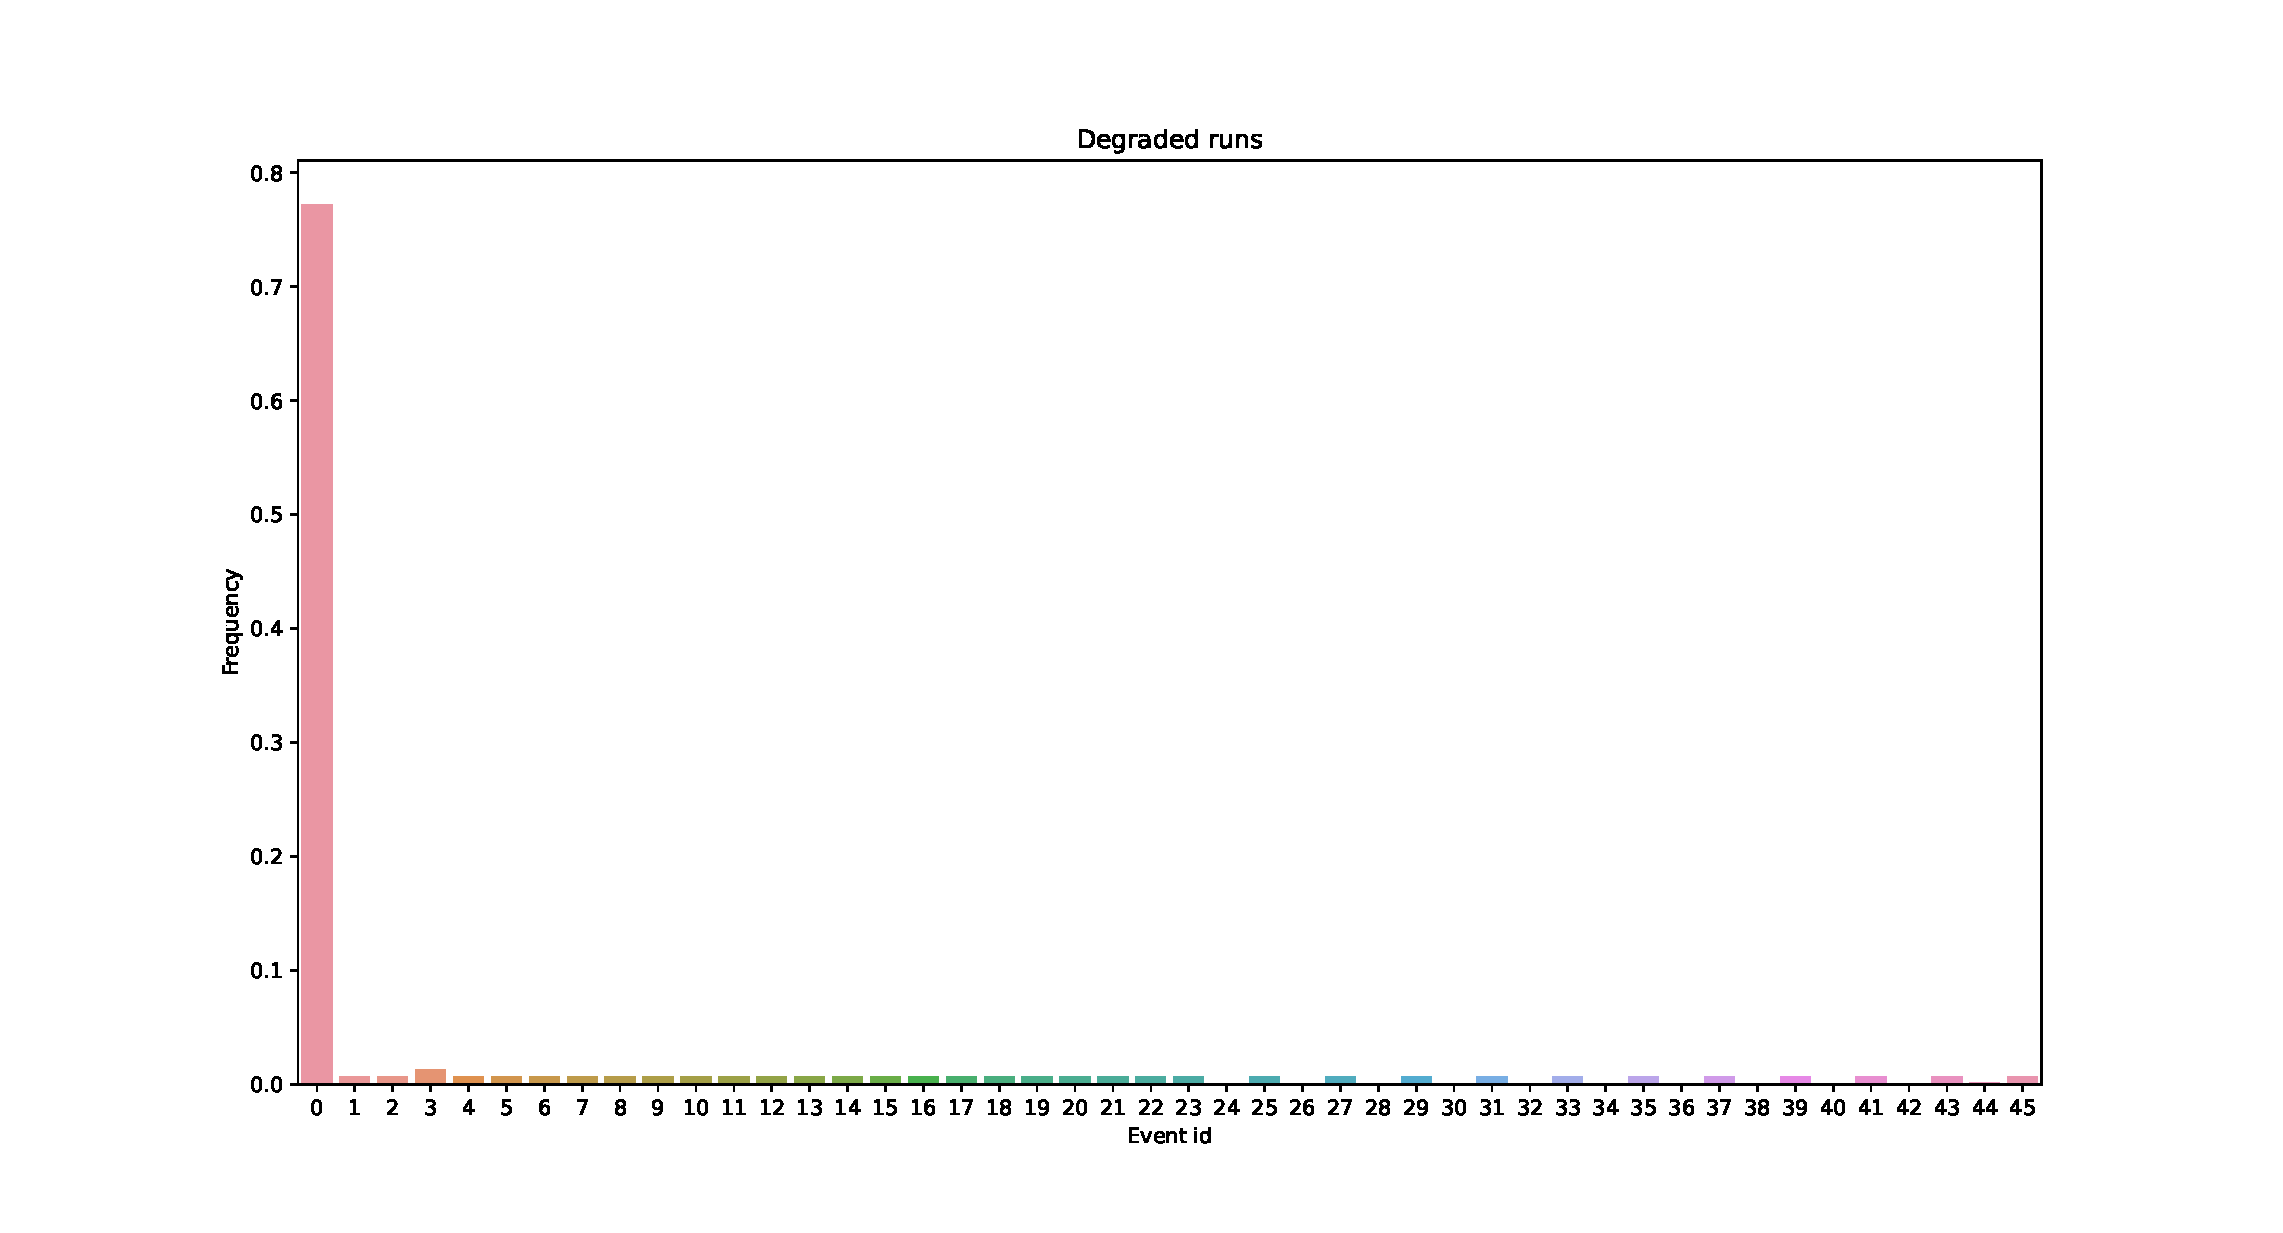
\includegraphics[width=8cm,keepaspectratio=true]{./degraded_runs_data_histogram.eps}
 \caption{Frequencies of events in degraded runs. The event id zero corresponds to the TICK event.}
 \label{figure:degraded_histogram}
\end{figure}

\begin{figure}[h]
 \centering
 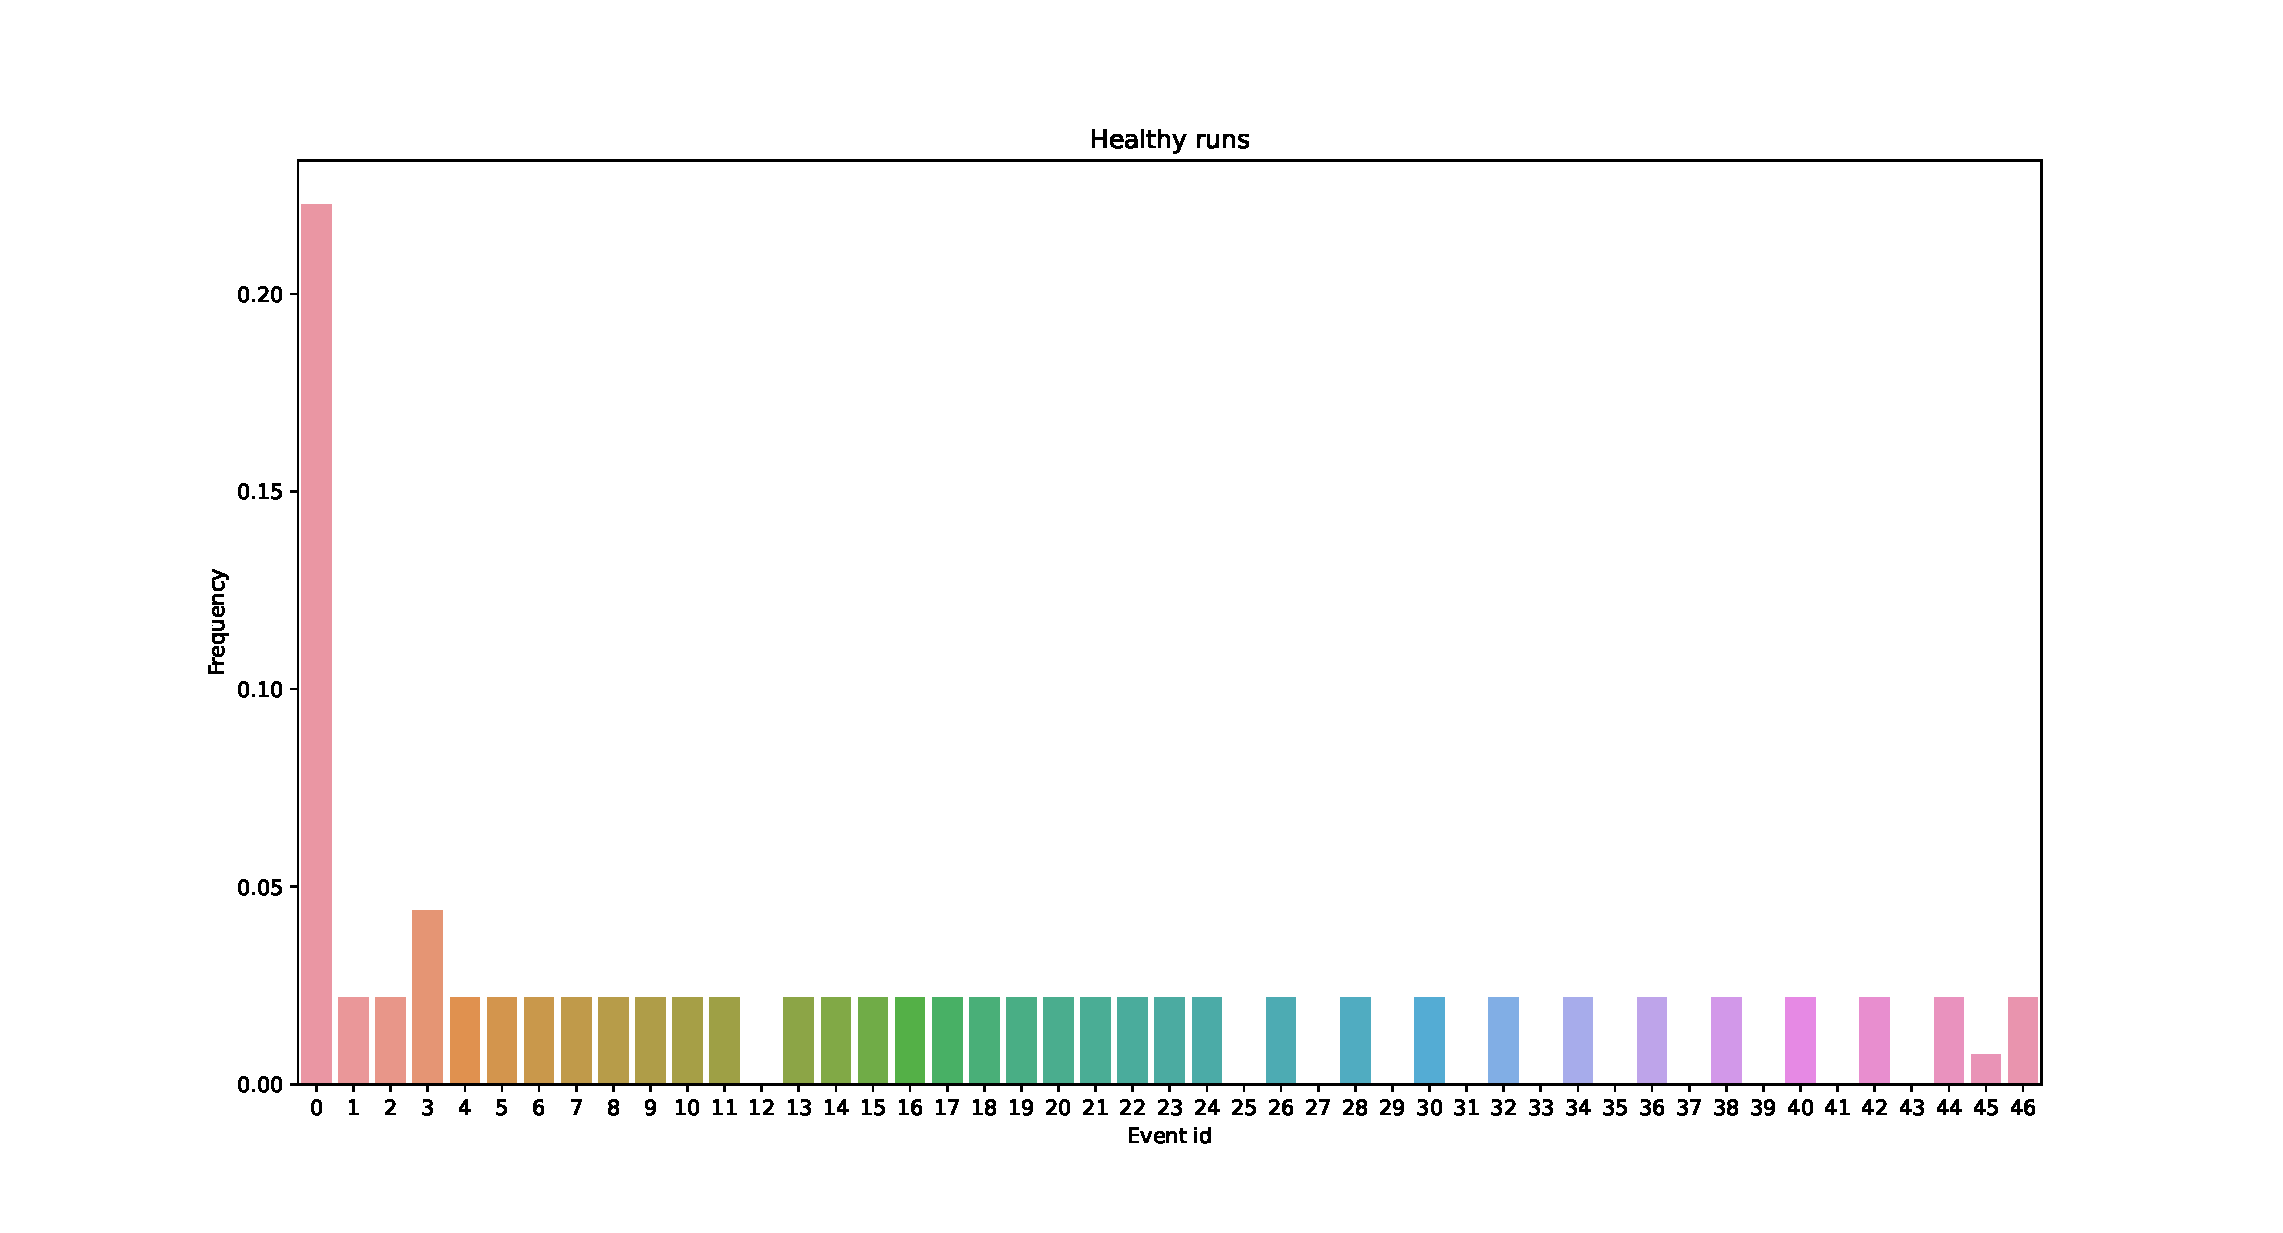
\includegraphics[width=8cm,keepaspectratio=true]{./healthy_runs_data_histogram.eps}
 \caption{Frequencies of events in healthy runs. The event id zero corresponds to the TICK event.}
 \label{figure:healthy_histogram}
\end{figure}

This is likely due to the fact that HMM is unable to perfectly model the causal relationships in the process traces, and that degraded sequences tend to have a higher frequency of ``TICK'' events (Figure \ref{figure:degraded_histogram}) in the traces designating the passing of time than in healthy sequences (Figure \ref{figure:healthy_histogram}). As ``TICK'' events are the most common event type in the training set as well, their respective probability is very high compared to other event types. This makes the HMM score healthy logs  lower than degraded logs.

When we graph the ROC AUC scores based on these log likelihoods across all the different numbers of hidden states (Figures \ref{figure:roc_log_likelihoods_10}, \ref{figure:roc_log_likelihoods_100} and \ref{figure:roc_log_likelihoods_1000}) we notice that the values are less than 0.5. This means that this model has negative predictiveness and we would do better if we inverted the predictions of the model to swap prediction to healthy when the model predicts degraded, and vice versa. However, it is not likely that this swap will generalize well to new fault types, so we will need to predict anomalous divergences differently.

We also notice that the number of hidden states doesn't seem to have a great effect.

Other research using HMMs for anomaly detection has found that naive scoring of the sequences doesn't work well for this purpose\cite{gornitz2015hidden}. Instead, they tend to suggest looking at the HMM hidden state sequences and differences of those to the healthy hidden state sequences.

In our case, the event ids are static across sequences, and the trained HMM model is static as well, so we can simply compare the hidden state sequences directly without the added complication of equivalence or similarity of different Hidden Markov Models. We simply compute histograms of hidden states in the observed window for the trained HMM, and compare the histograms to the histograms of the training set using KL divergence.

Doing the same for KL divergences (0 means perfect distributional match of the observed HMM hidden state distribution to the training data hidden state distribution, and larger values denote worse match) shows that some of the degraded runs do indeed have worse KL divergences than the KL divergences for the healthy runs. See Figures \ref{figure:kl_10}, \ref{figure:kl_100} and \ref{figure:kl_1000}.

When we graph the ROC AUC scores based on these KL divergences across all the different numbers of hidden states (Figures \ref{figure:roc_kl_10}, \ref{figure:roc_kl_100} and \ref{figure:roc_kl_1000}), we notice that the number of hidden states doesn't seem to have a great effect here either as long as there are at least 2 hidden states.

The discrimination rate for the model when the cut-off score is set to the maximal divergence for the healthy samples, that is, for no false positives, is about 1\% and at most 5\% for sequence length of 10 (Figure \ref{figure:discrimination_rate_10}). It is about 6\% and at most 9\% for the sequence length of 100 (Figure \ref{figure:discrimination_rate_100}), and about 8\% and at most 15\% for the sequence length of 1000 (Figure \ref{figure:discrimination_rate_1000}).


\bibliographystyle{IEEEtran}
\bibliography{results}

\begin{IEEEbiography}[{
\includegraphics[width=1in,height=1.25in,clip,keepaspectratio]{tero}}]{Tero Keski-Valkama}
Tero Keski-Valkama is working as a lead ML \& AI engineer in HERE Switzerland GmbH. He has been programming neural networks since high school in 1990s.
\end{IEEEbiography}

\appendices

\section{Diagrams}

\begin{figure}[h]
 \centering
 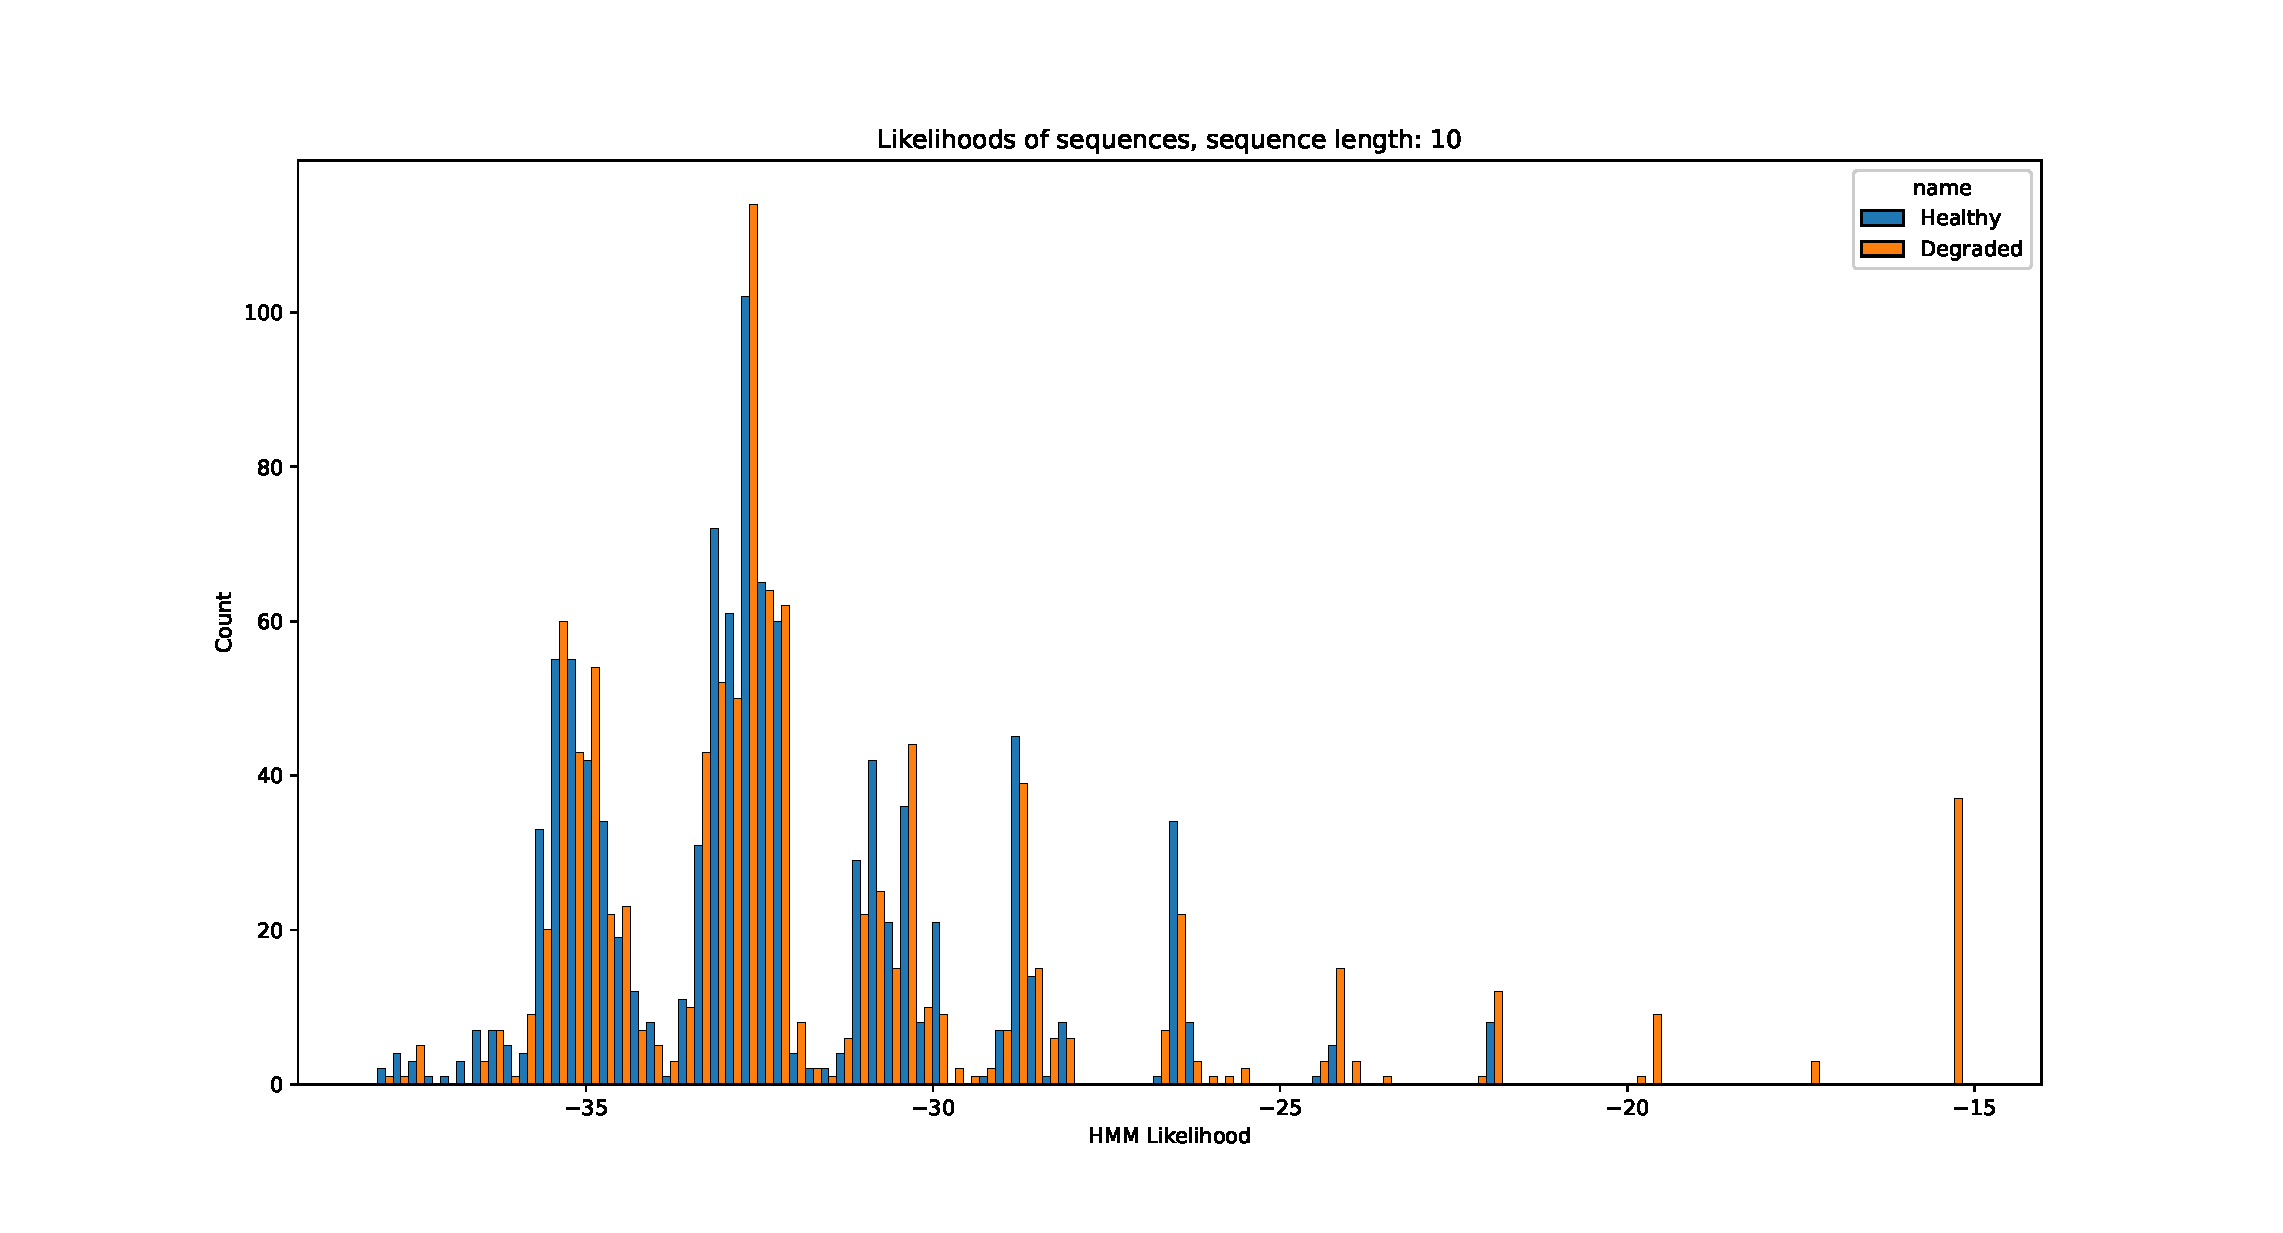
\includegraphics[width=10cm,keepaspectratio=true]{./hmm_histograms_10.eps}
 \caption{Counts of different HMM log likelihood scores for both healthy and degraded runs, sequence length 10 and 6 hidden states.}
 \label{figure:log_likelihood_10}
\end{figure}

\begin{figure}[h]
 \centering
 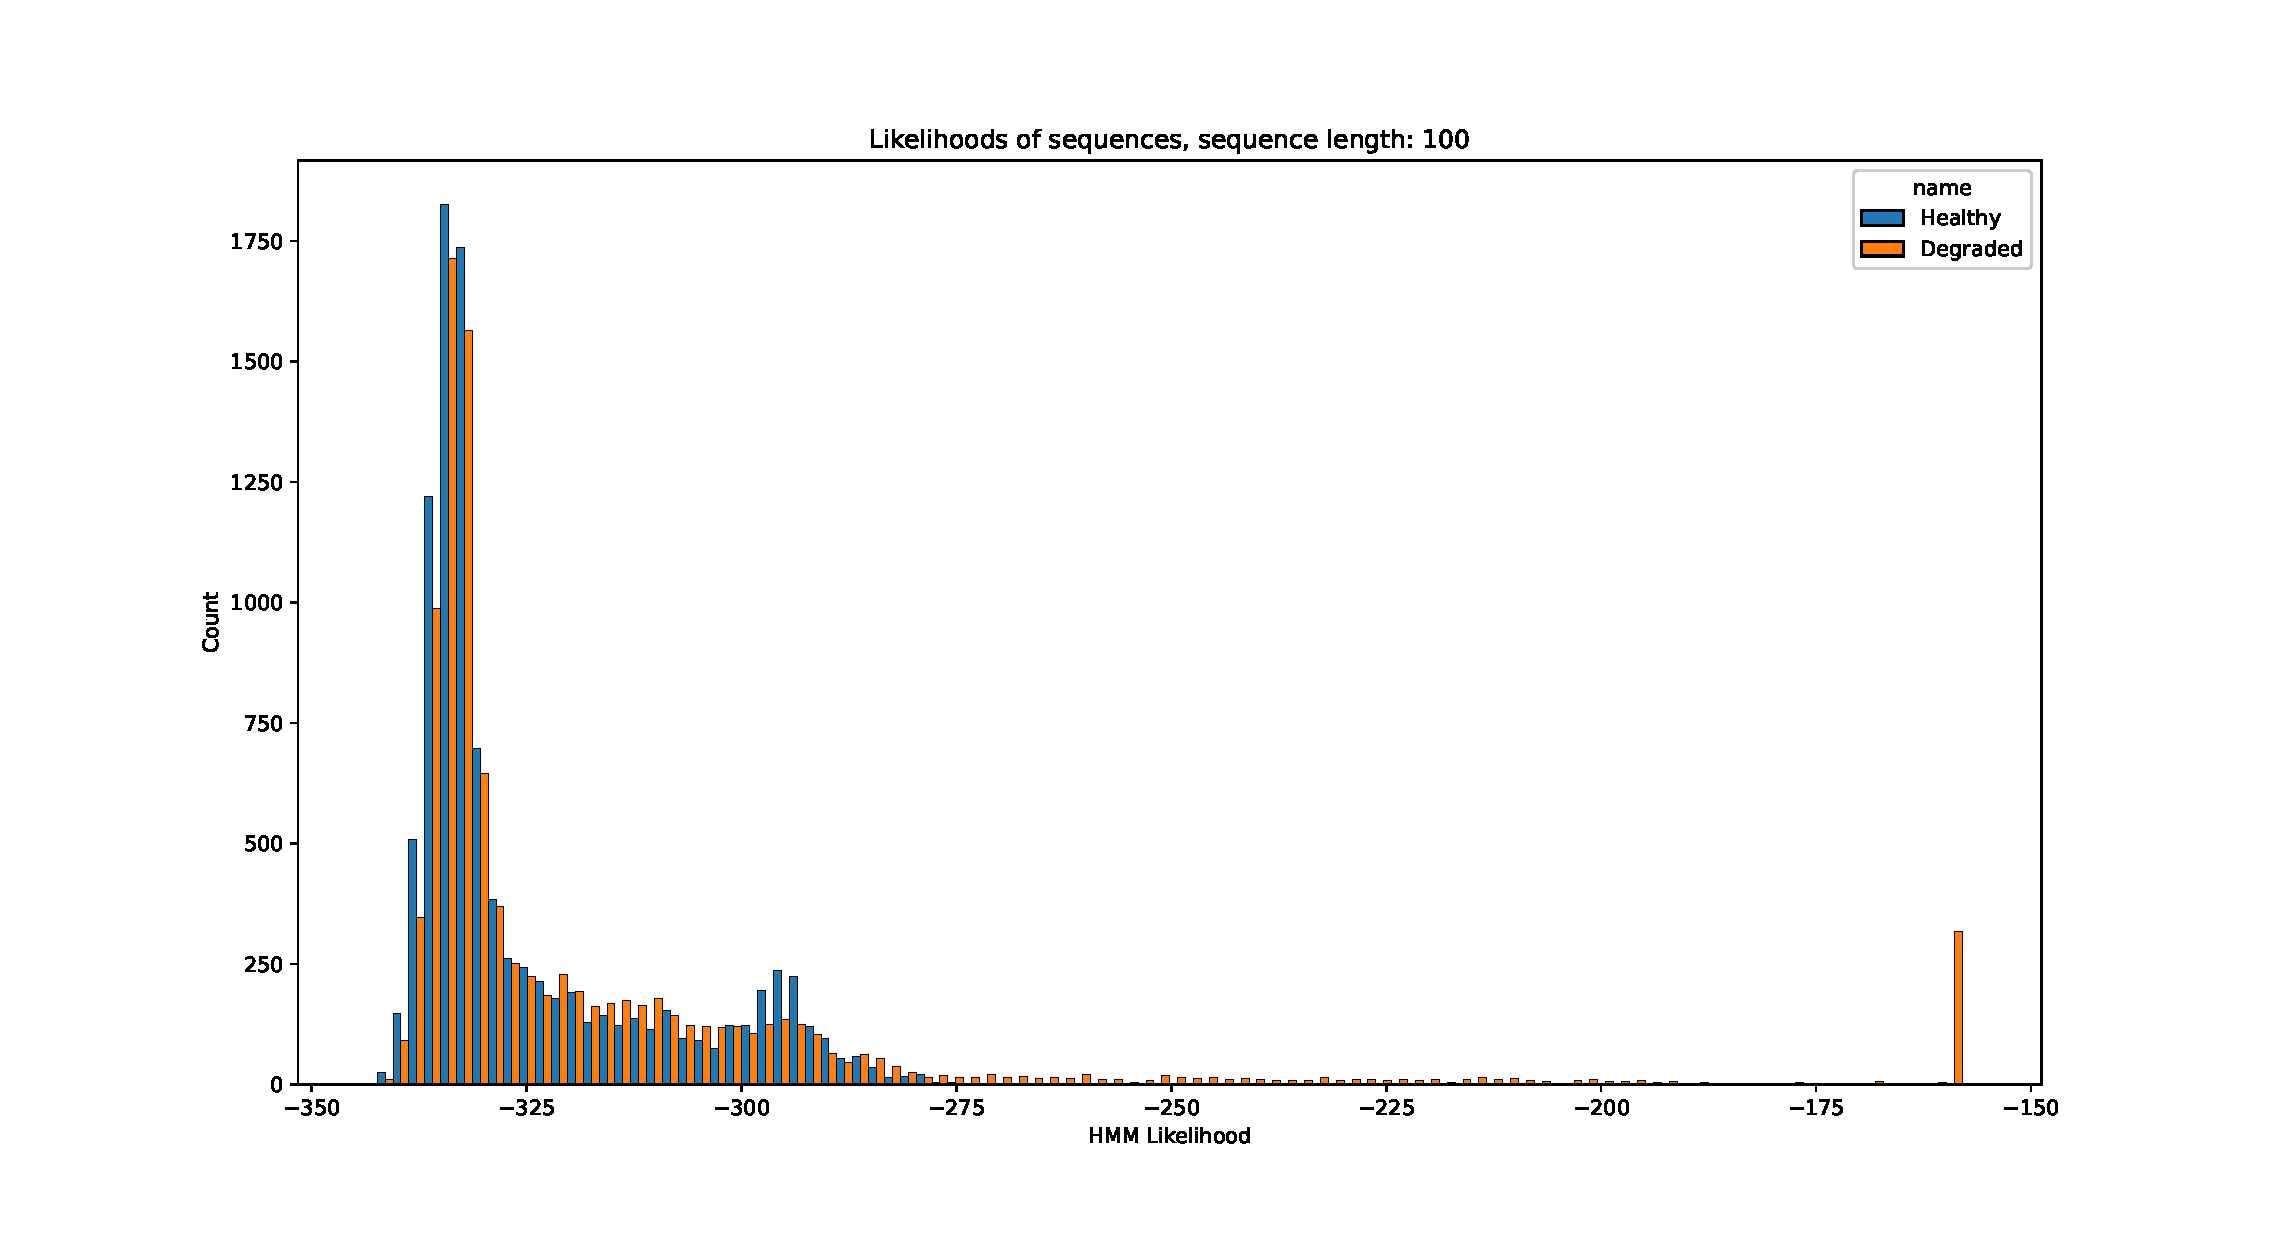
\includegraphics[width=10cm,keepaspectratio=true]{./hmm_histograms_100.eps}
 \caption{Counts of different HMM log likelihood scores for both healthy and degraded runs, sequence length 100 and 6 hidden states.}
 \label{figure:log_likelihood_100}
\end{figure}

\begin{figure}[h]
 \centering
 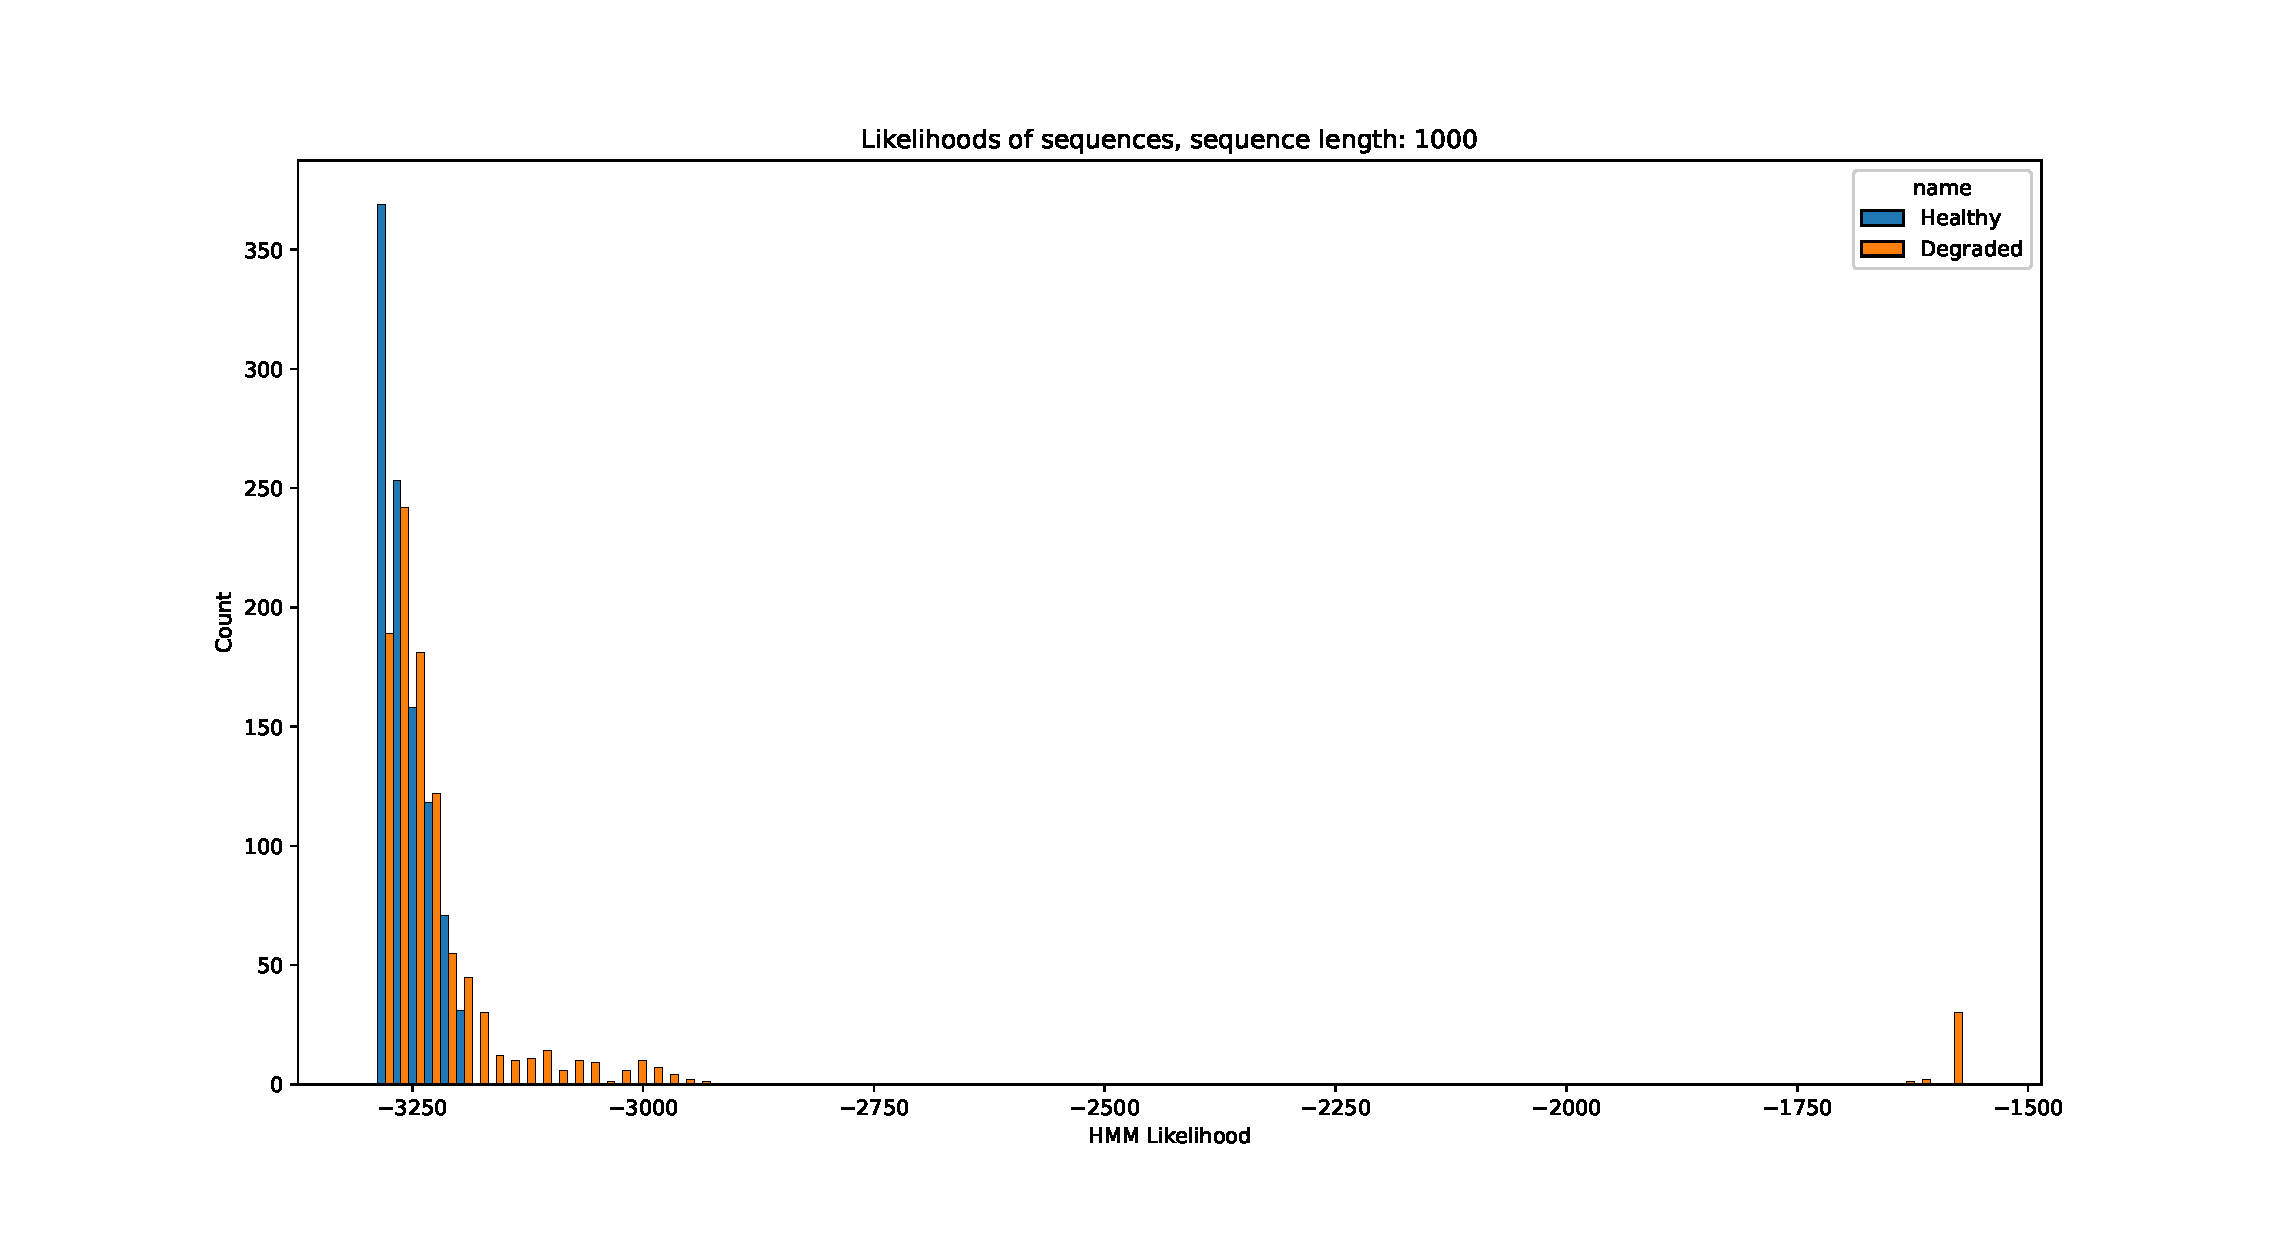
\includegraphics[width=10cm,keepaspectratio=true]{./hmm_histograms_1000.eps}
 \caption{Counts of different HMM log likelihood scores for both healthy and degraded runs, sequence length 1000 and 6 hidden states.}
 \label{figure:log_likelihood_1000}
\end{figure}

\begin{figure}[h]
 \centering
 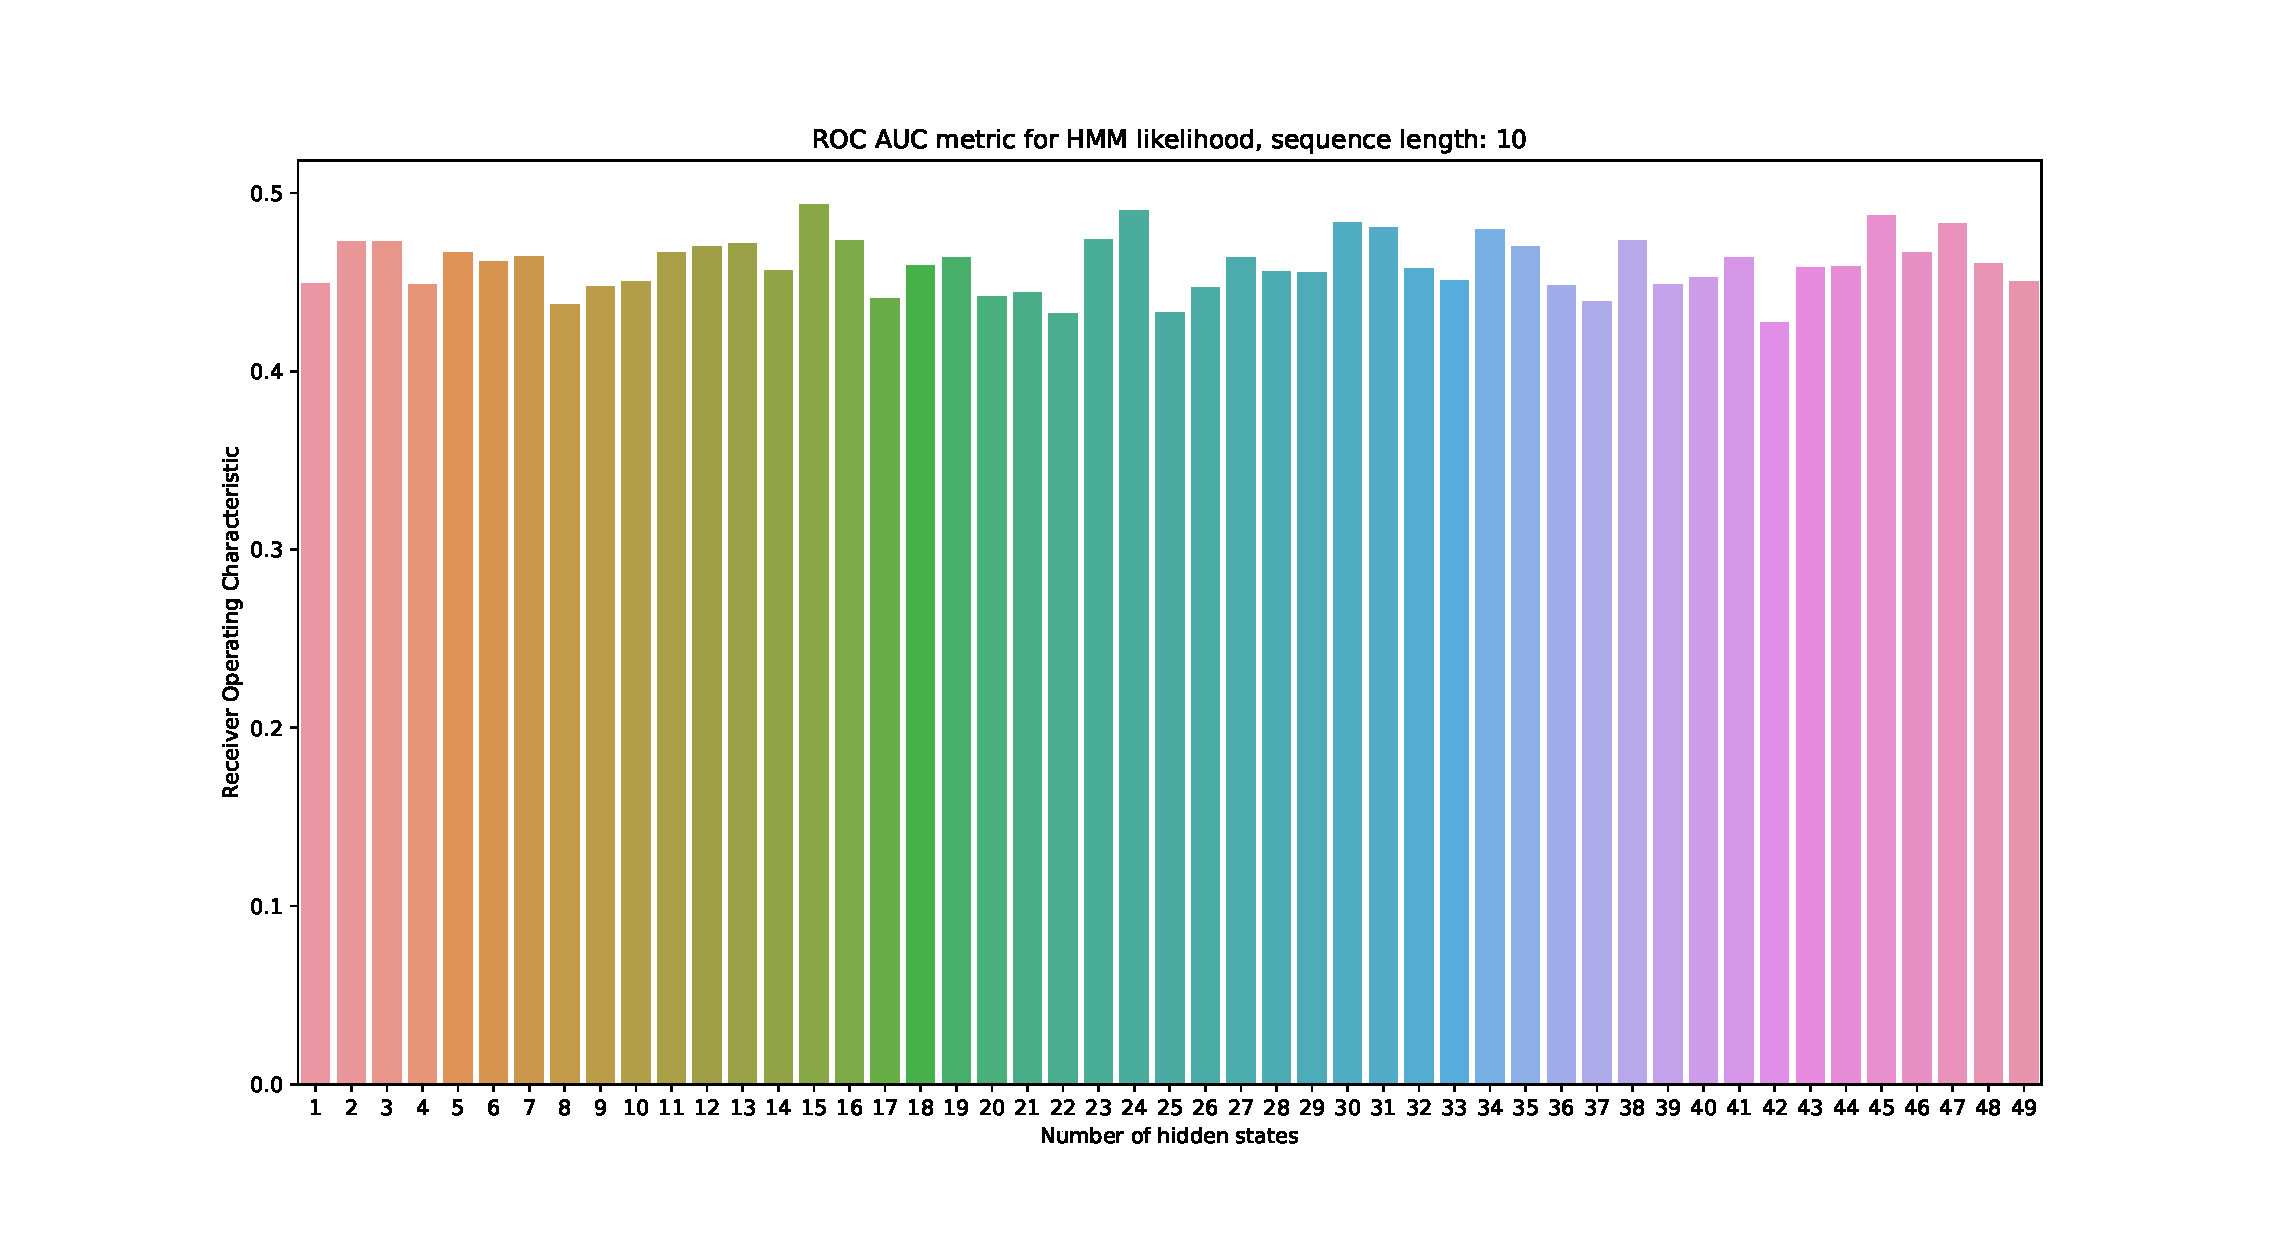
\includegraphics[width=10cm,keepaspectratio=true]{./roc_hmm_score_10.eps}
 \caption{Receiver Operating Characteristic AUC scores for different numbers of hidden states used using HMM log likelihood scores with a sequence length of 10.}
 \label{figure:roc_log_likelihoods_10}
\end{figure}

\begin{figure}[h]
 \centering
 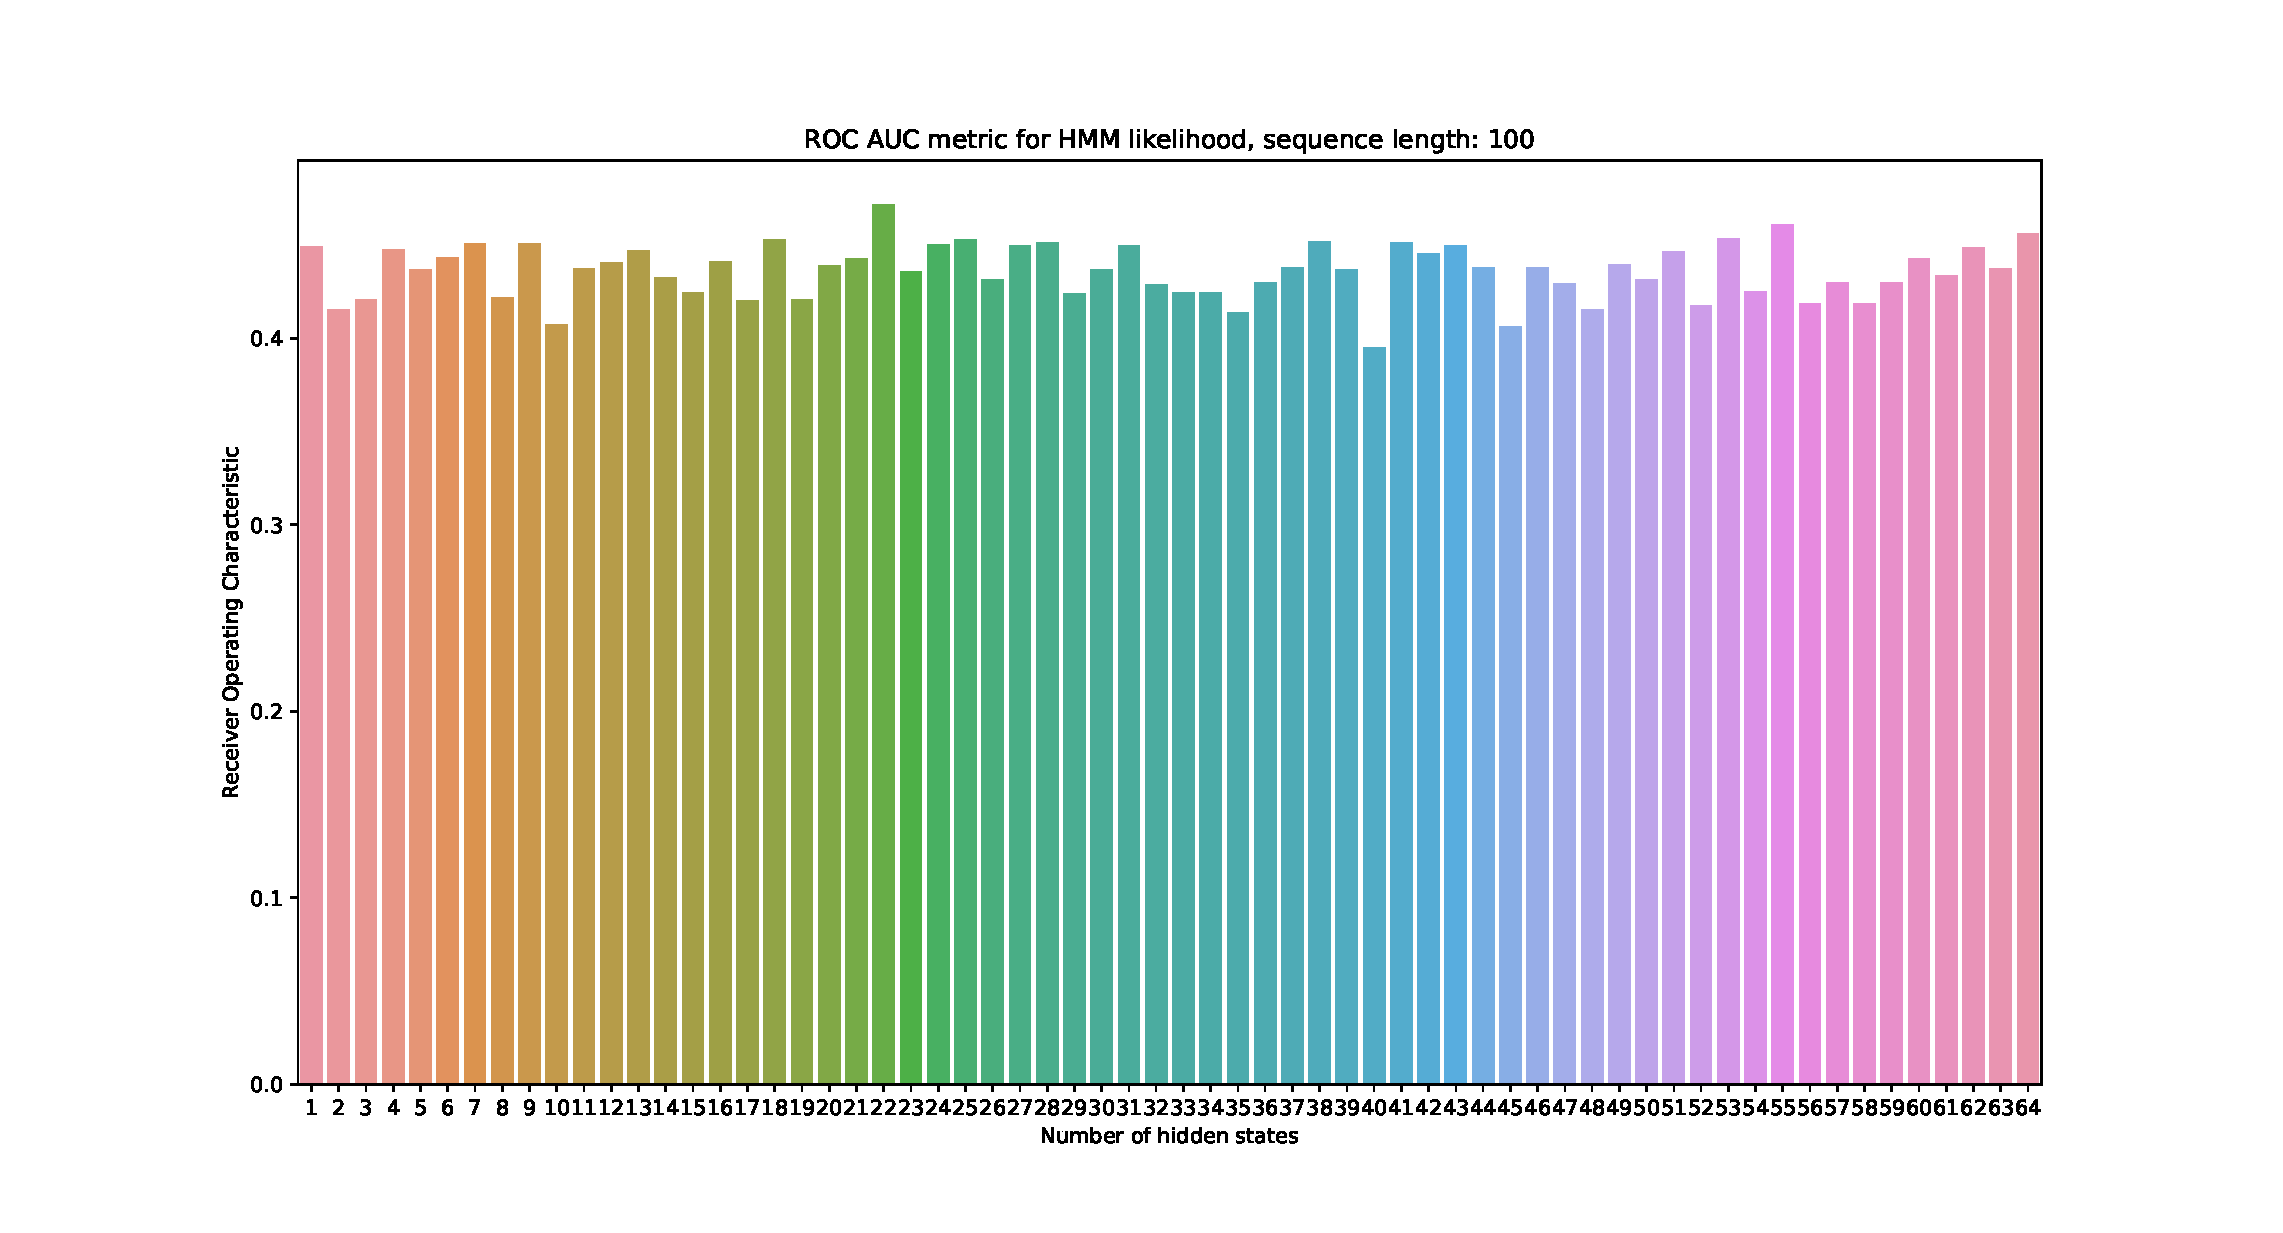
\includegraphics[width=10cm,keepaspectratio=true]{./roc_hmm_score_100.eps}
 \caption{Receiver Operating Characteristic AUC scores for different numbers of hidden states used using HMM log likelihood scores with a sequence length of 100.}
 \label{figure:roc_log_likelihoods_100}
\end{figure}

\begin{figure}[h]
 \centering
 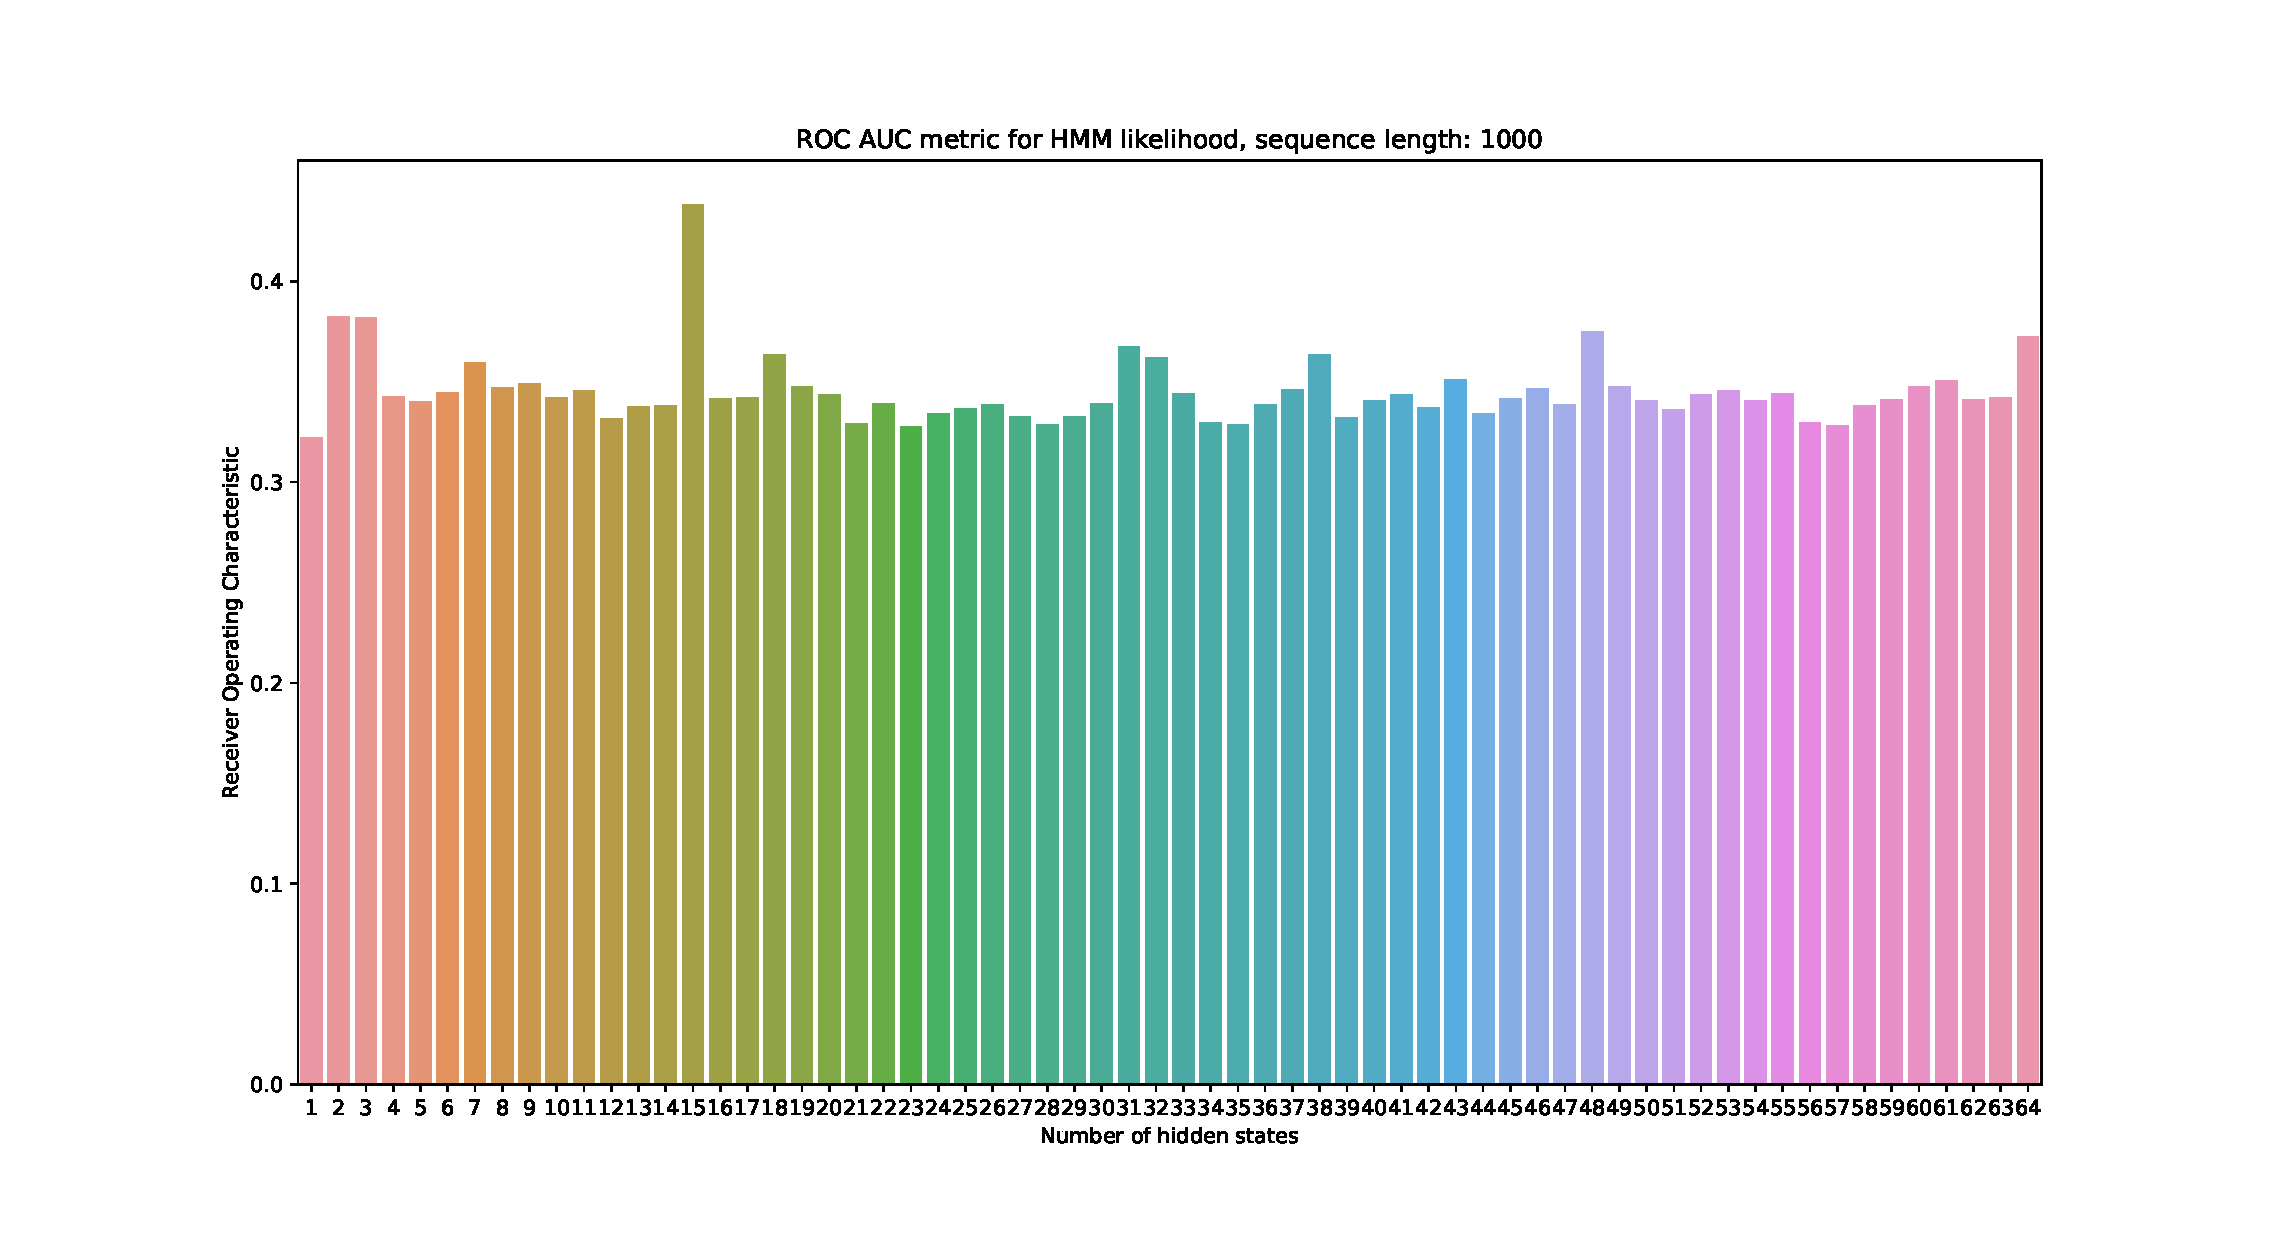
\includegraphics[width=10cm,keepaspectratio=true]{./roc_hmm_score_1000.eps}
 \caption{Receiver Operating Characteristic AUC scores for different numbers of hidden states used using HMM log likelihood scores with a sequence length of 1000.}
 \label{figure:roc_log_likelihoods_1000}
\end{figure}

\begin{figure}[h]
 \centering
 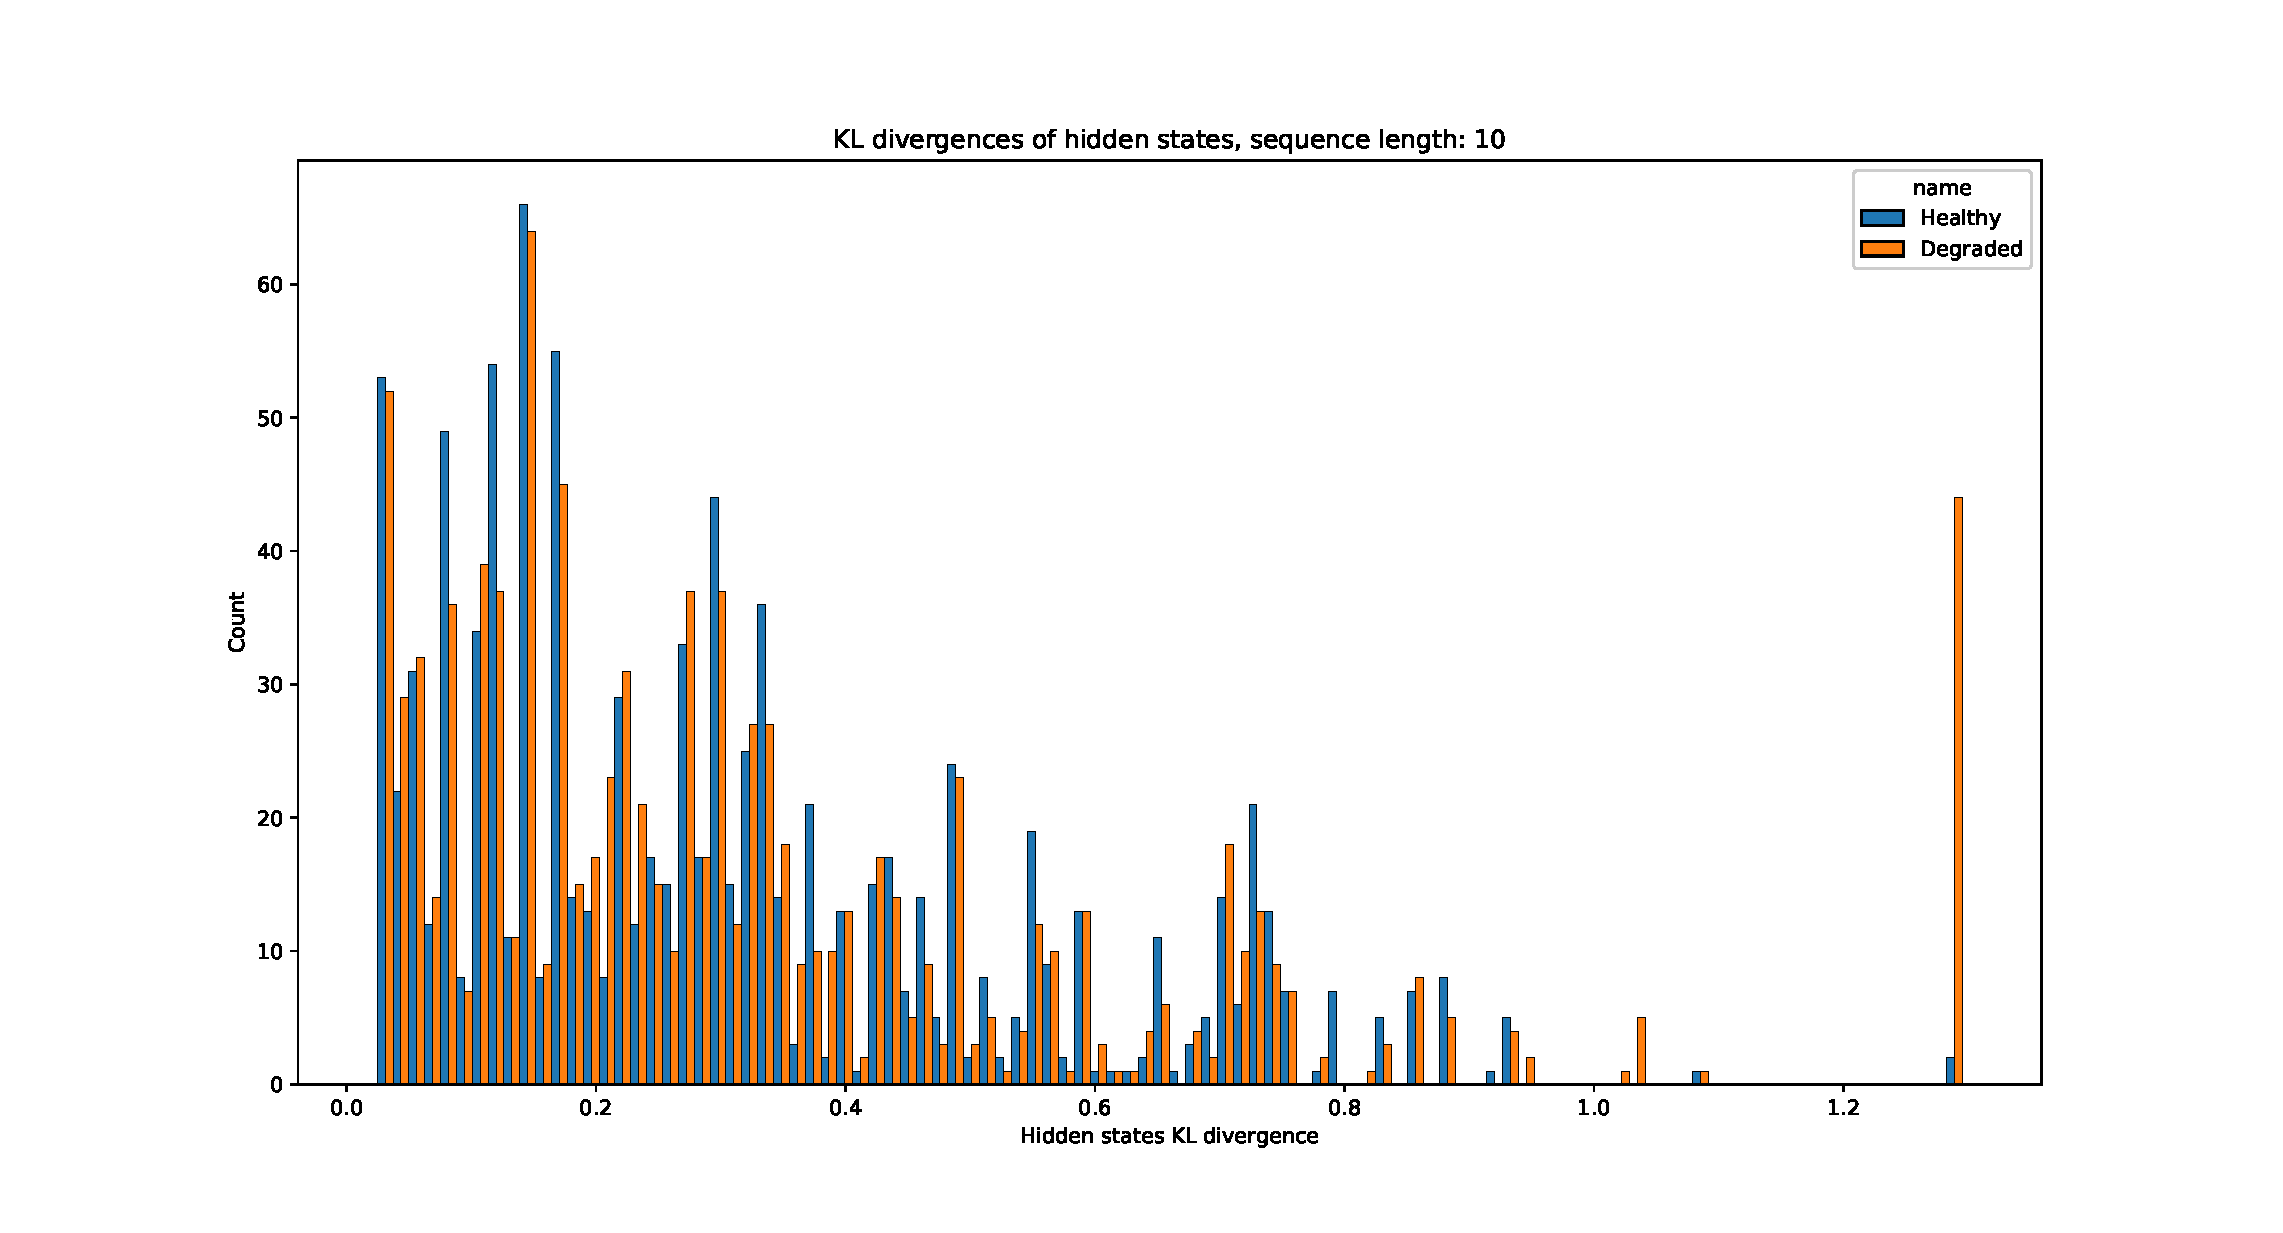
\includegraphics[width=10cm,keepaspectratio=true]{./kl_histograms_10.eps}
 \caption{Counts of different HMM hidden state KL divergences for both healthy and degraded runs, sequence length 10 and 6 hidden states.}
 \label{figure:kl_10}
\end{figure}

\begin{figure}[h]
 \centering
 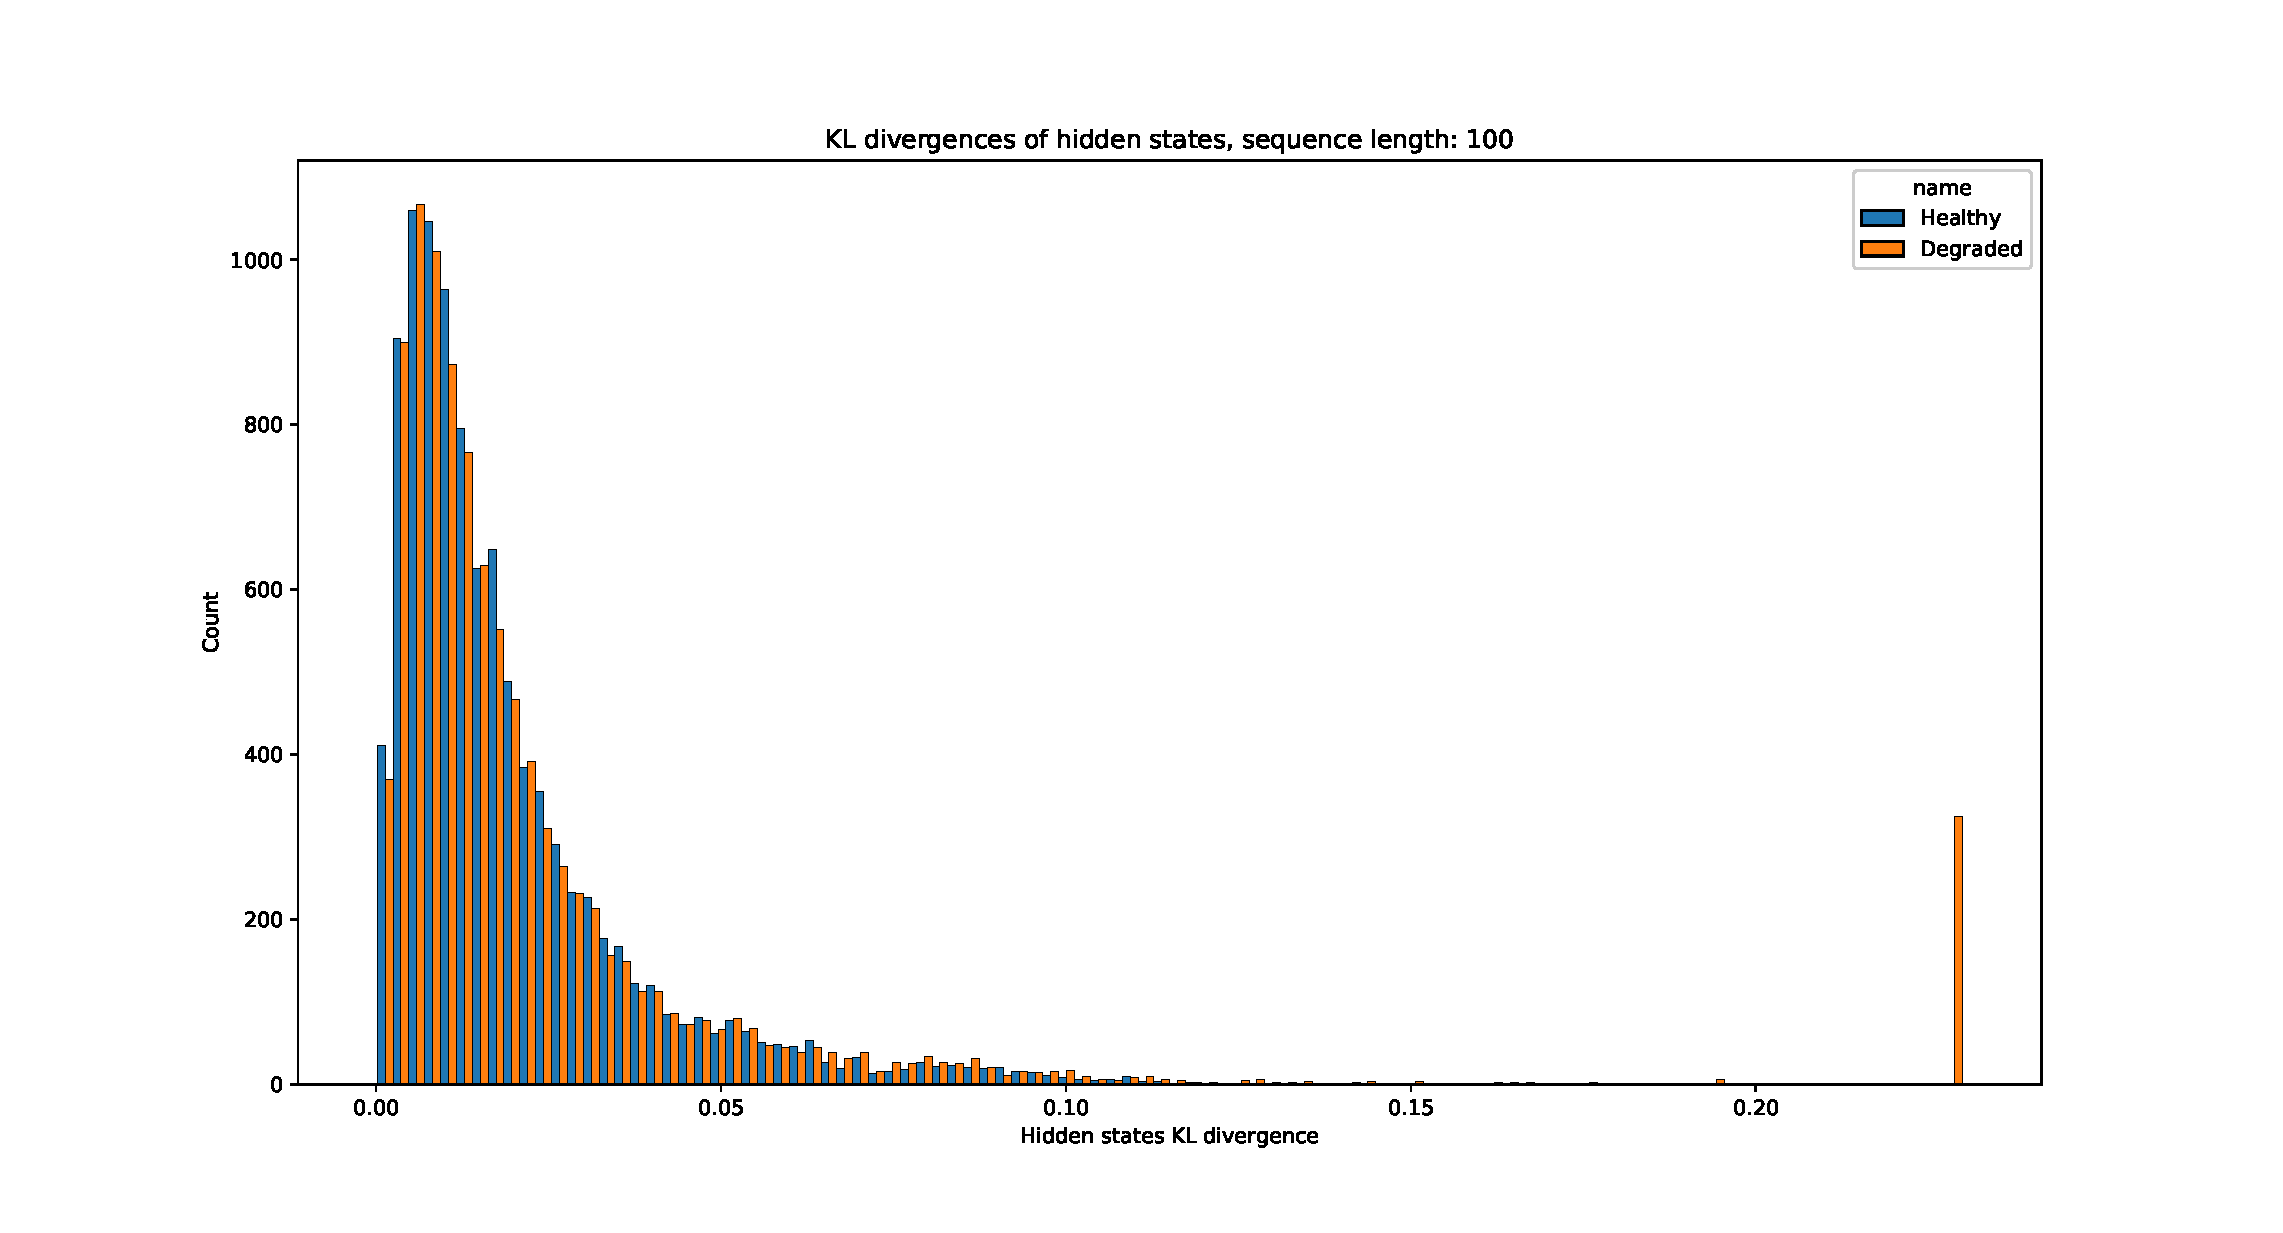
\includegraphics[width=10cm,keepaspectratio=true]{./kl_histograms_100.eps}
 \caption{Counts of different HMM hidden state KL divergences for both healthy and degraded runs, sequence length 100 and 6 hidden states.}
 \label{figure:kl_100}
\end{figure}

\begin{figure}[h]
 \centering
 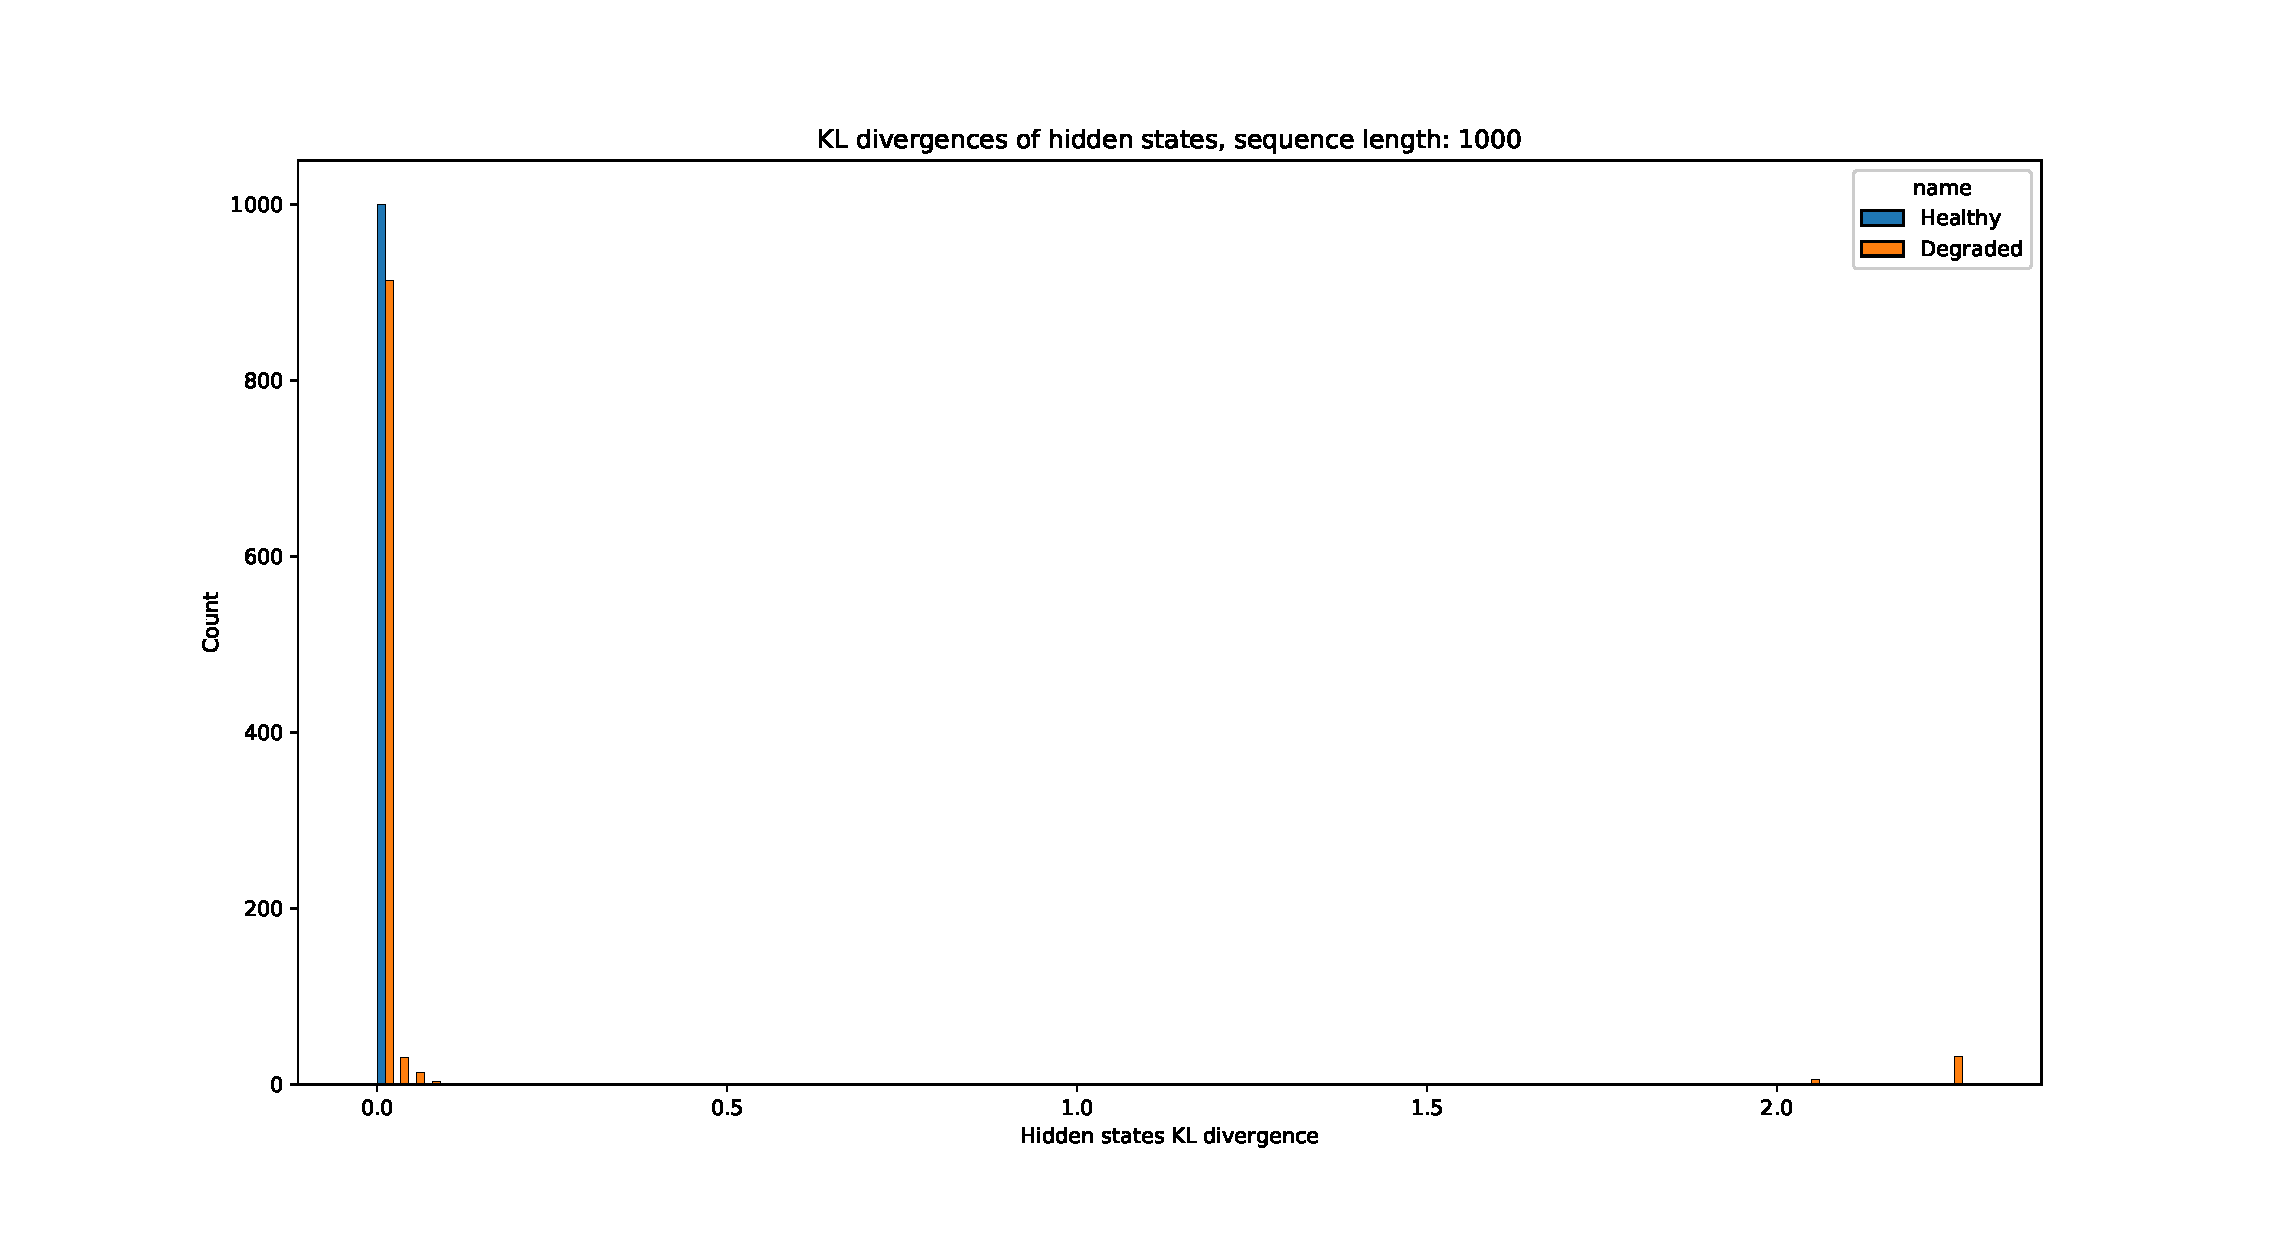
\includegraphics[width=10cm,keepaspectratio=true]{./kl_histograms_1000.eps}
 \caption{Counts of different HMM hidden state KL divergences for both healthy and degraded runs, sequence length 1000 and 6 hidden states.}
 \label{figure:kl_1000}
\end{figure}

\begin{figure}[h]
 \centering
 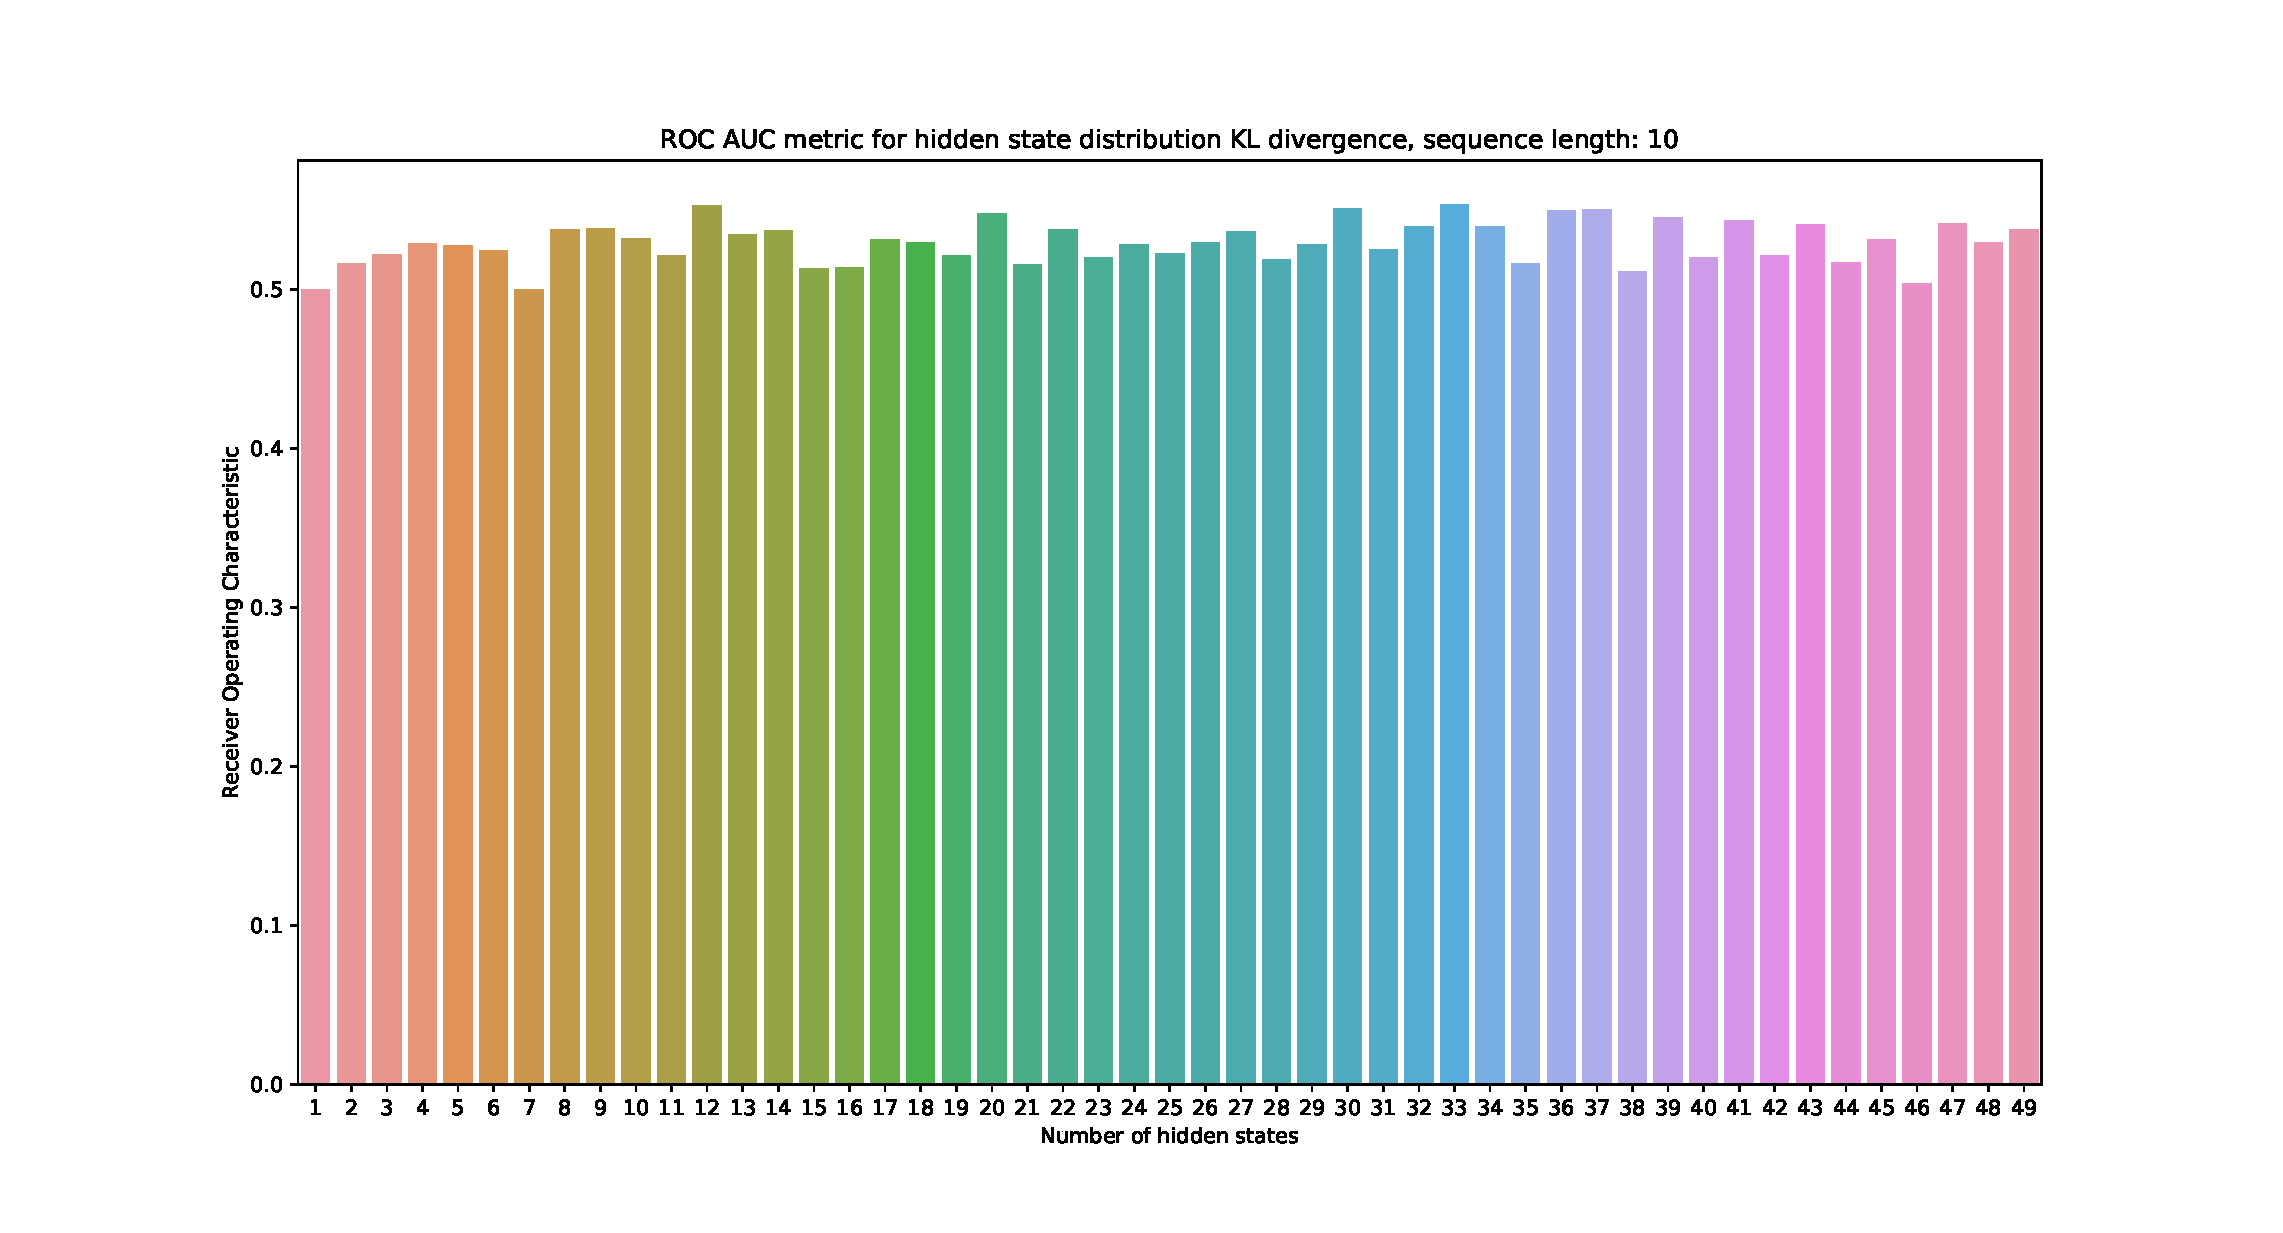
\includegraphics[width=10cm,keepaspectratio=true]{./roc_kl_score_10.eps}
 \caption{Receiver Operating Characteristic AUC scores for different numbers of hidden states used using HMM hidden state KL divergence scores with a sequence length of 10.}
 \label{figure:roc_kl_10}
\end{figure}

\begin{figure}[h]
 \centering
 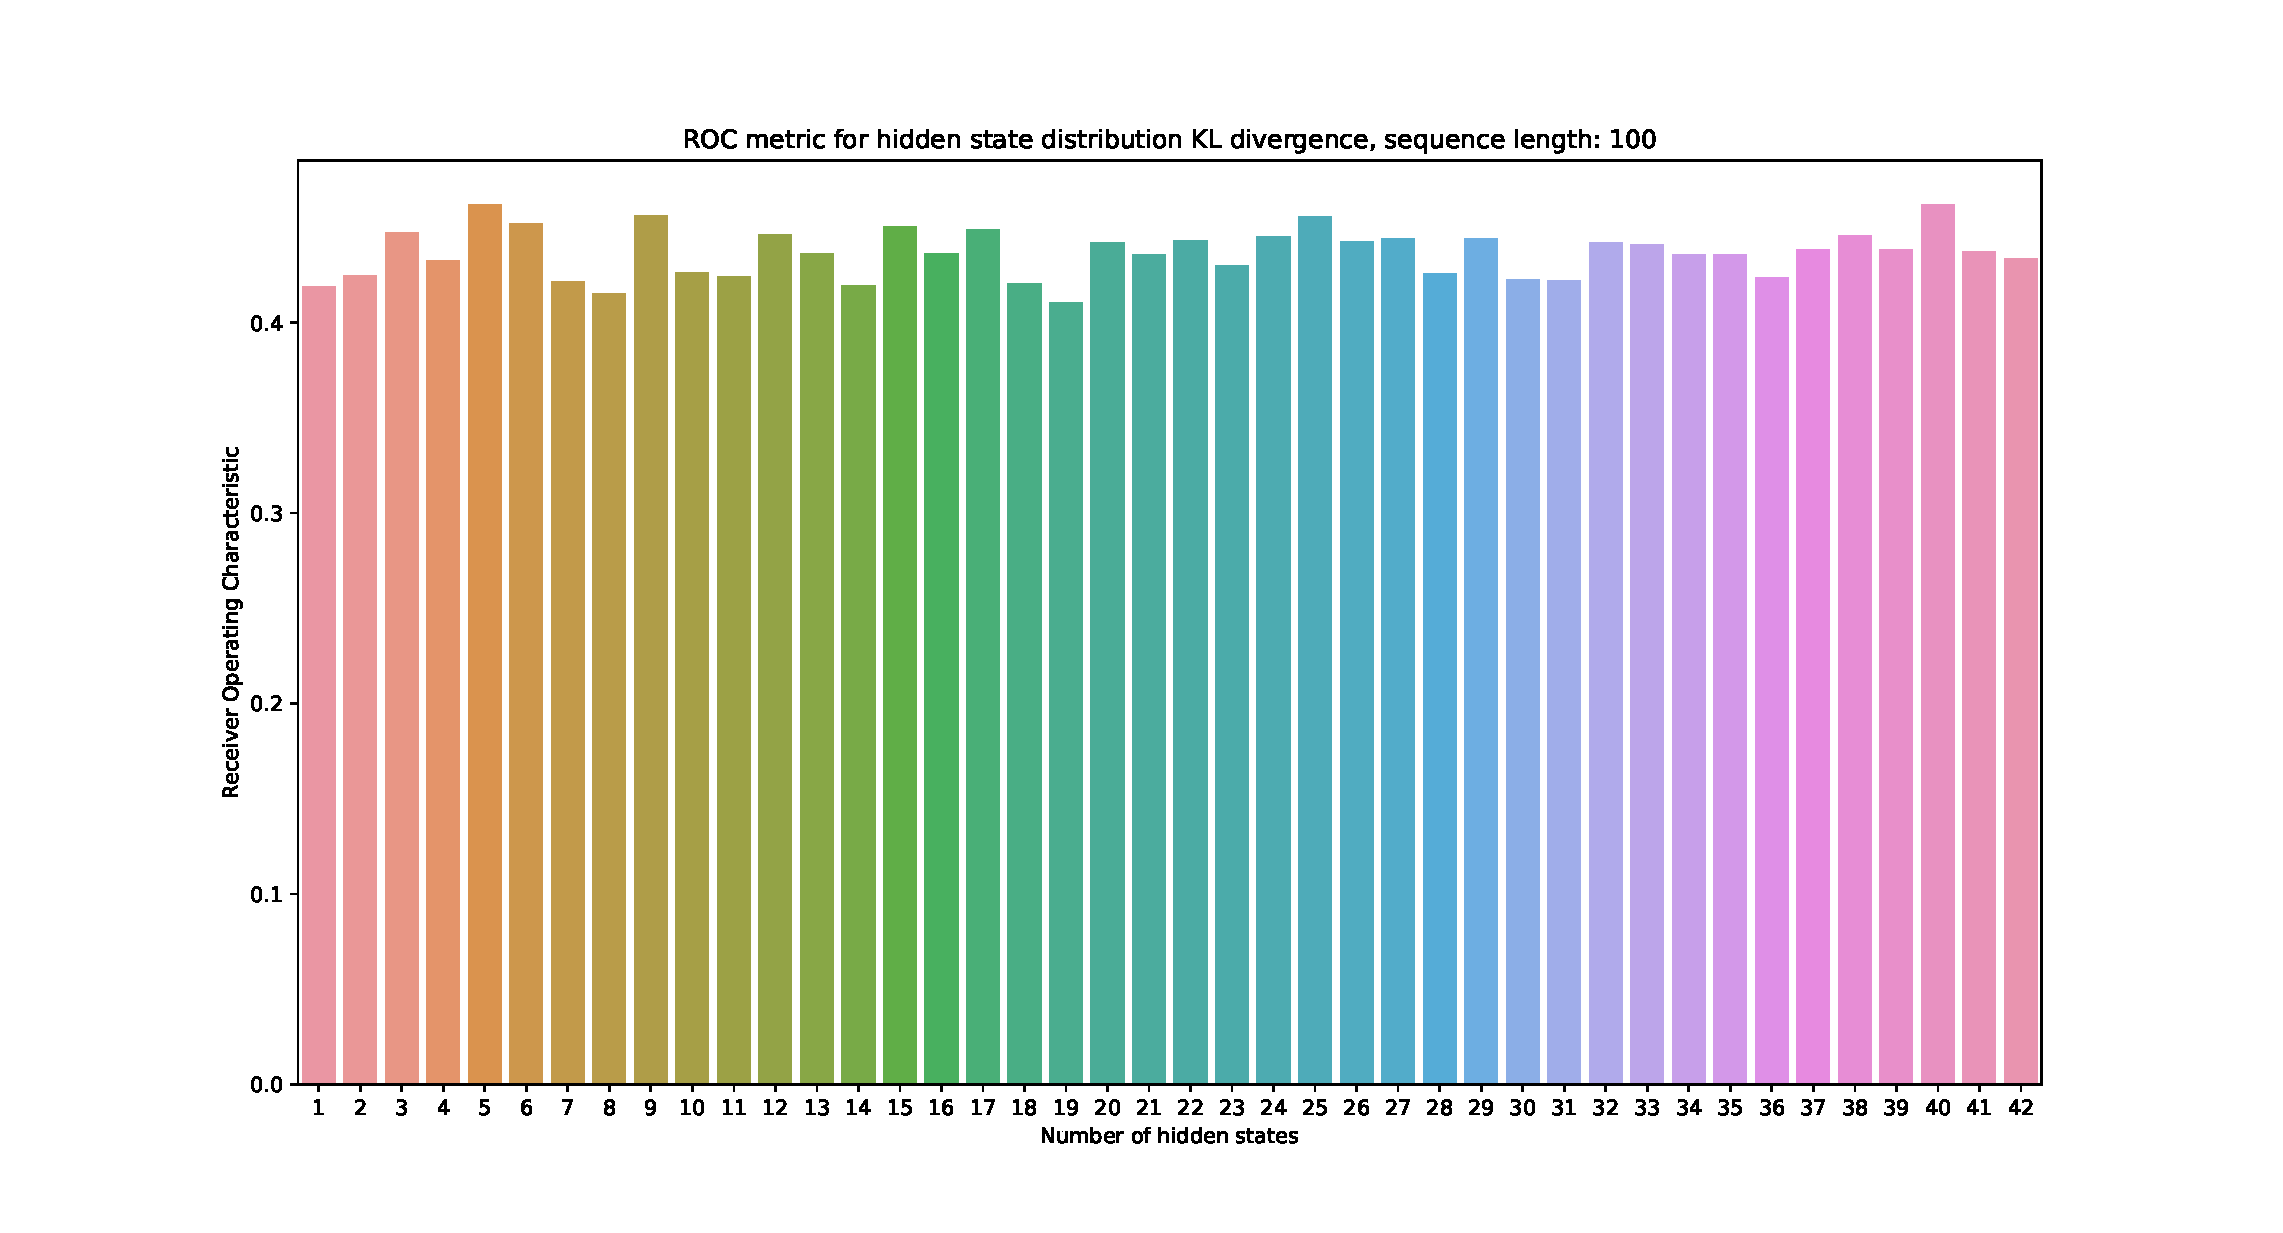
\includegraphics[width=10cm,keepaspectratio=true]{./roc_kl_score_100.eps}
 \caption{Receiver Operating Characteristic AUC scores for different numbers of hidden states used using HMM hidden state KL divergence scores with a sequence length of 100.}
 \label{figure:roc_kl_100}
\end{figure}

\begin{figure}[h]
 \centering
 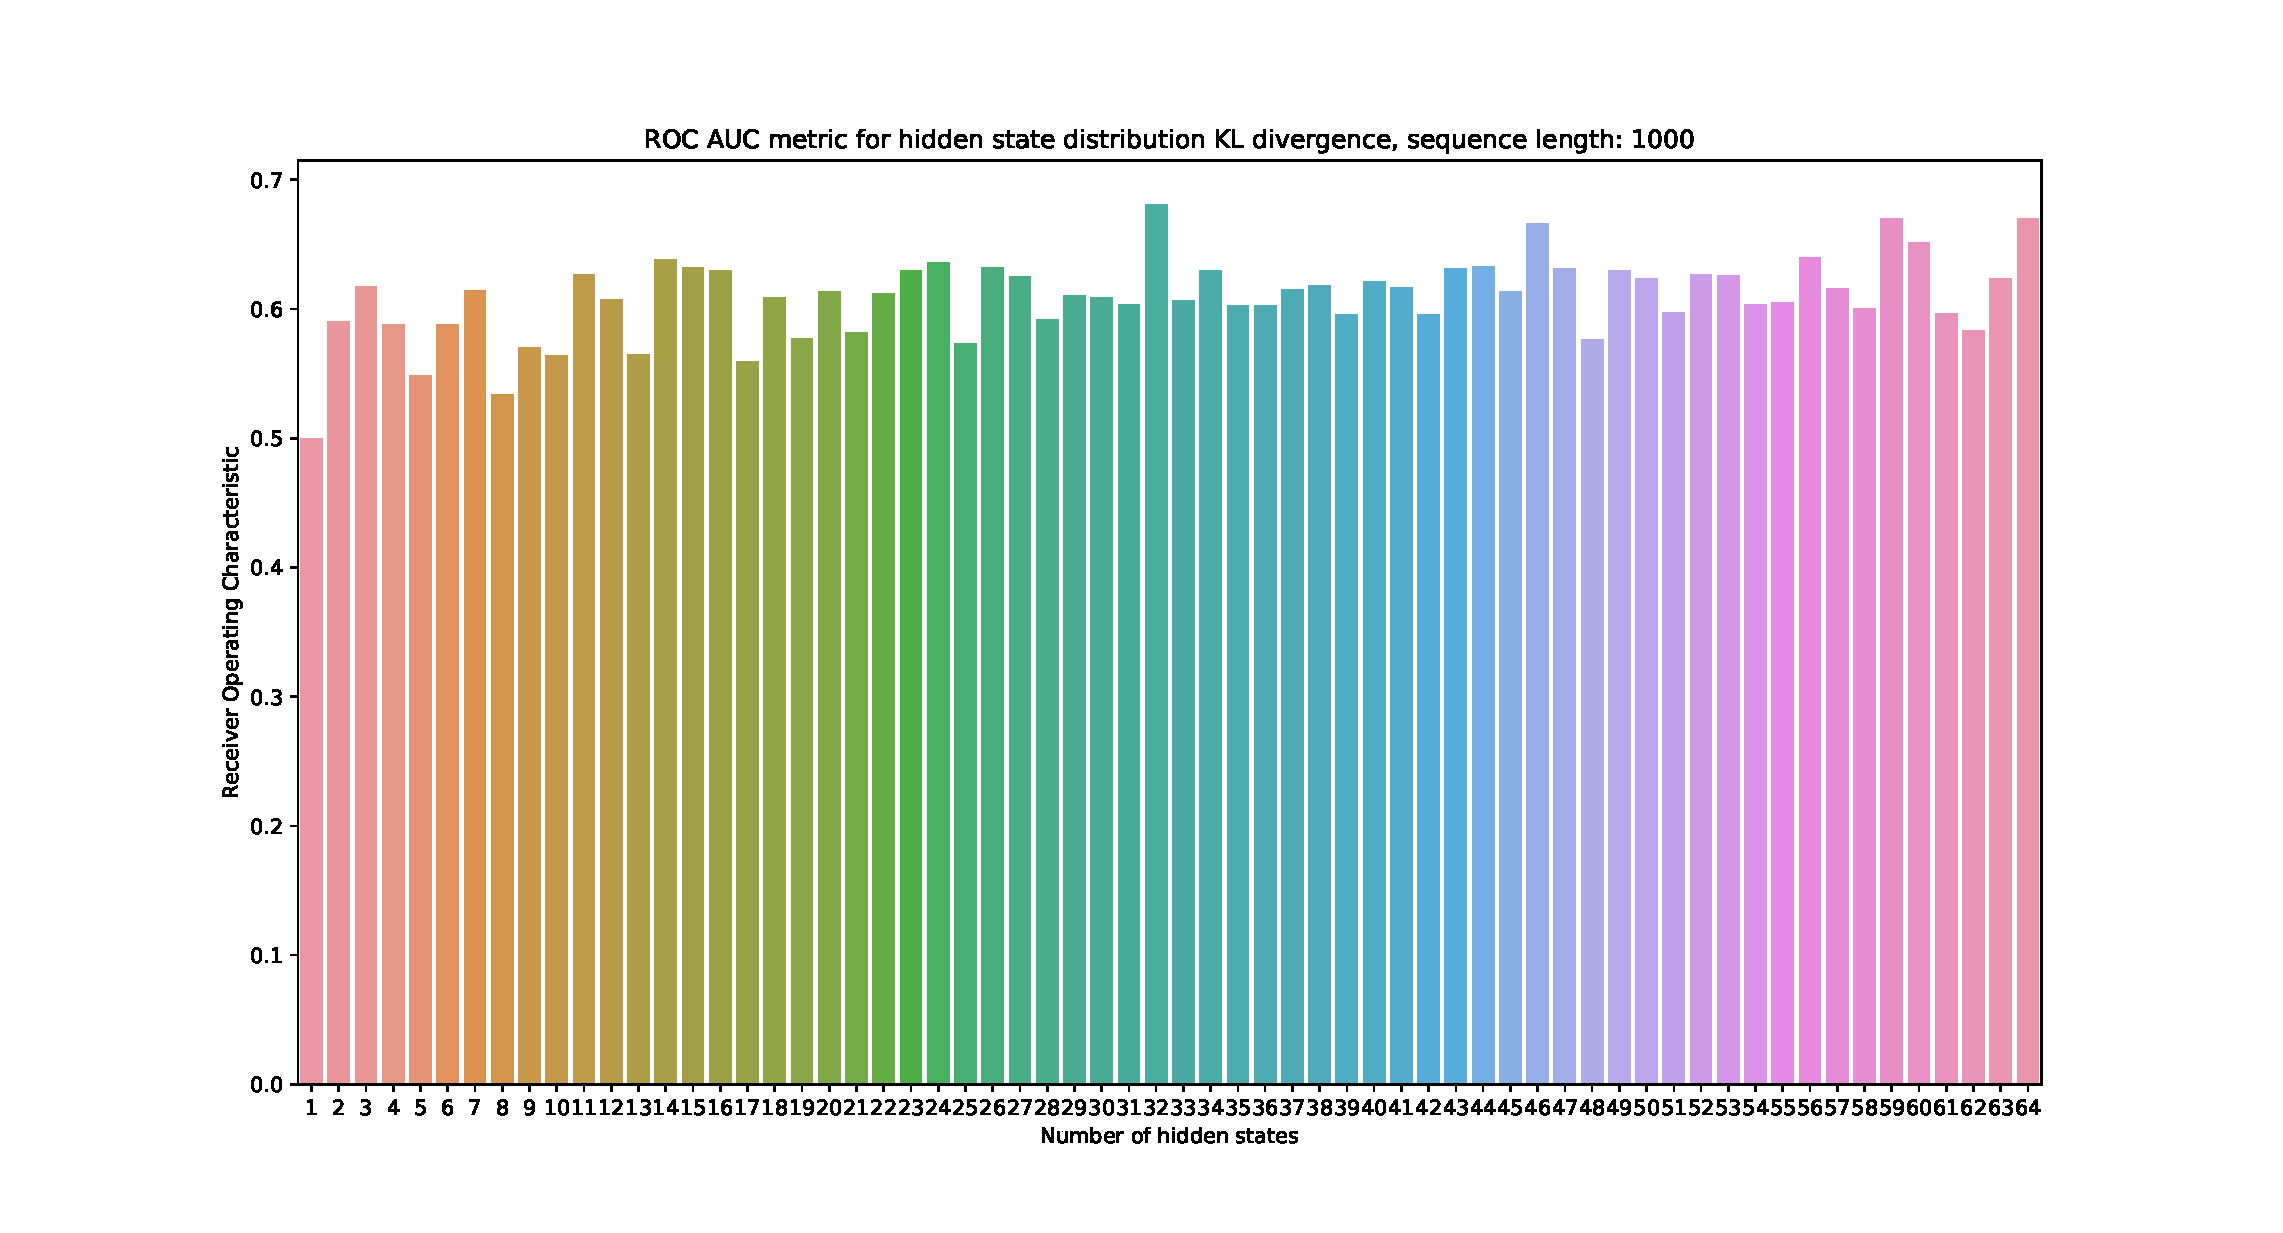
\includegraphics[width=10cm,keepaspectratio=true]{./roc_kl_score_1000.eps}
 \caption{Receiver Operating Characteristic AUC scores for different numbers of hidden states used using HMM hidden state KL divergence scores with a sequence length of 1000.}
 \label{figure:roc_kl_1000}
\end{figure}

\begin{figure}[h]
 \centering
 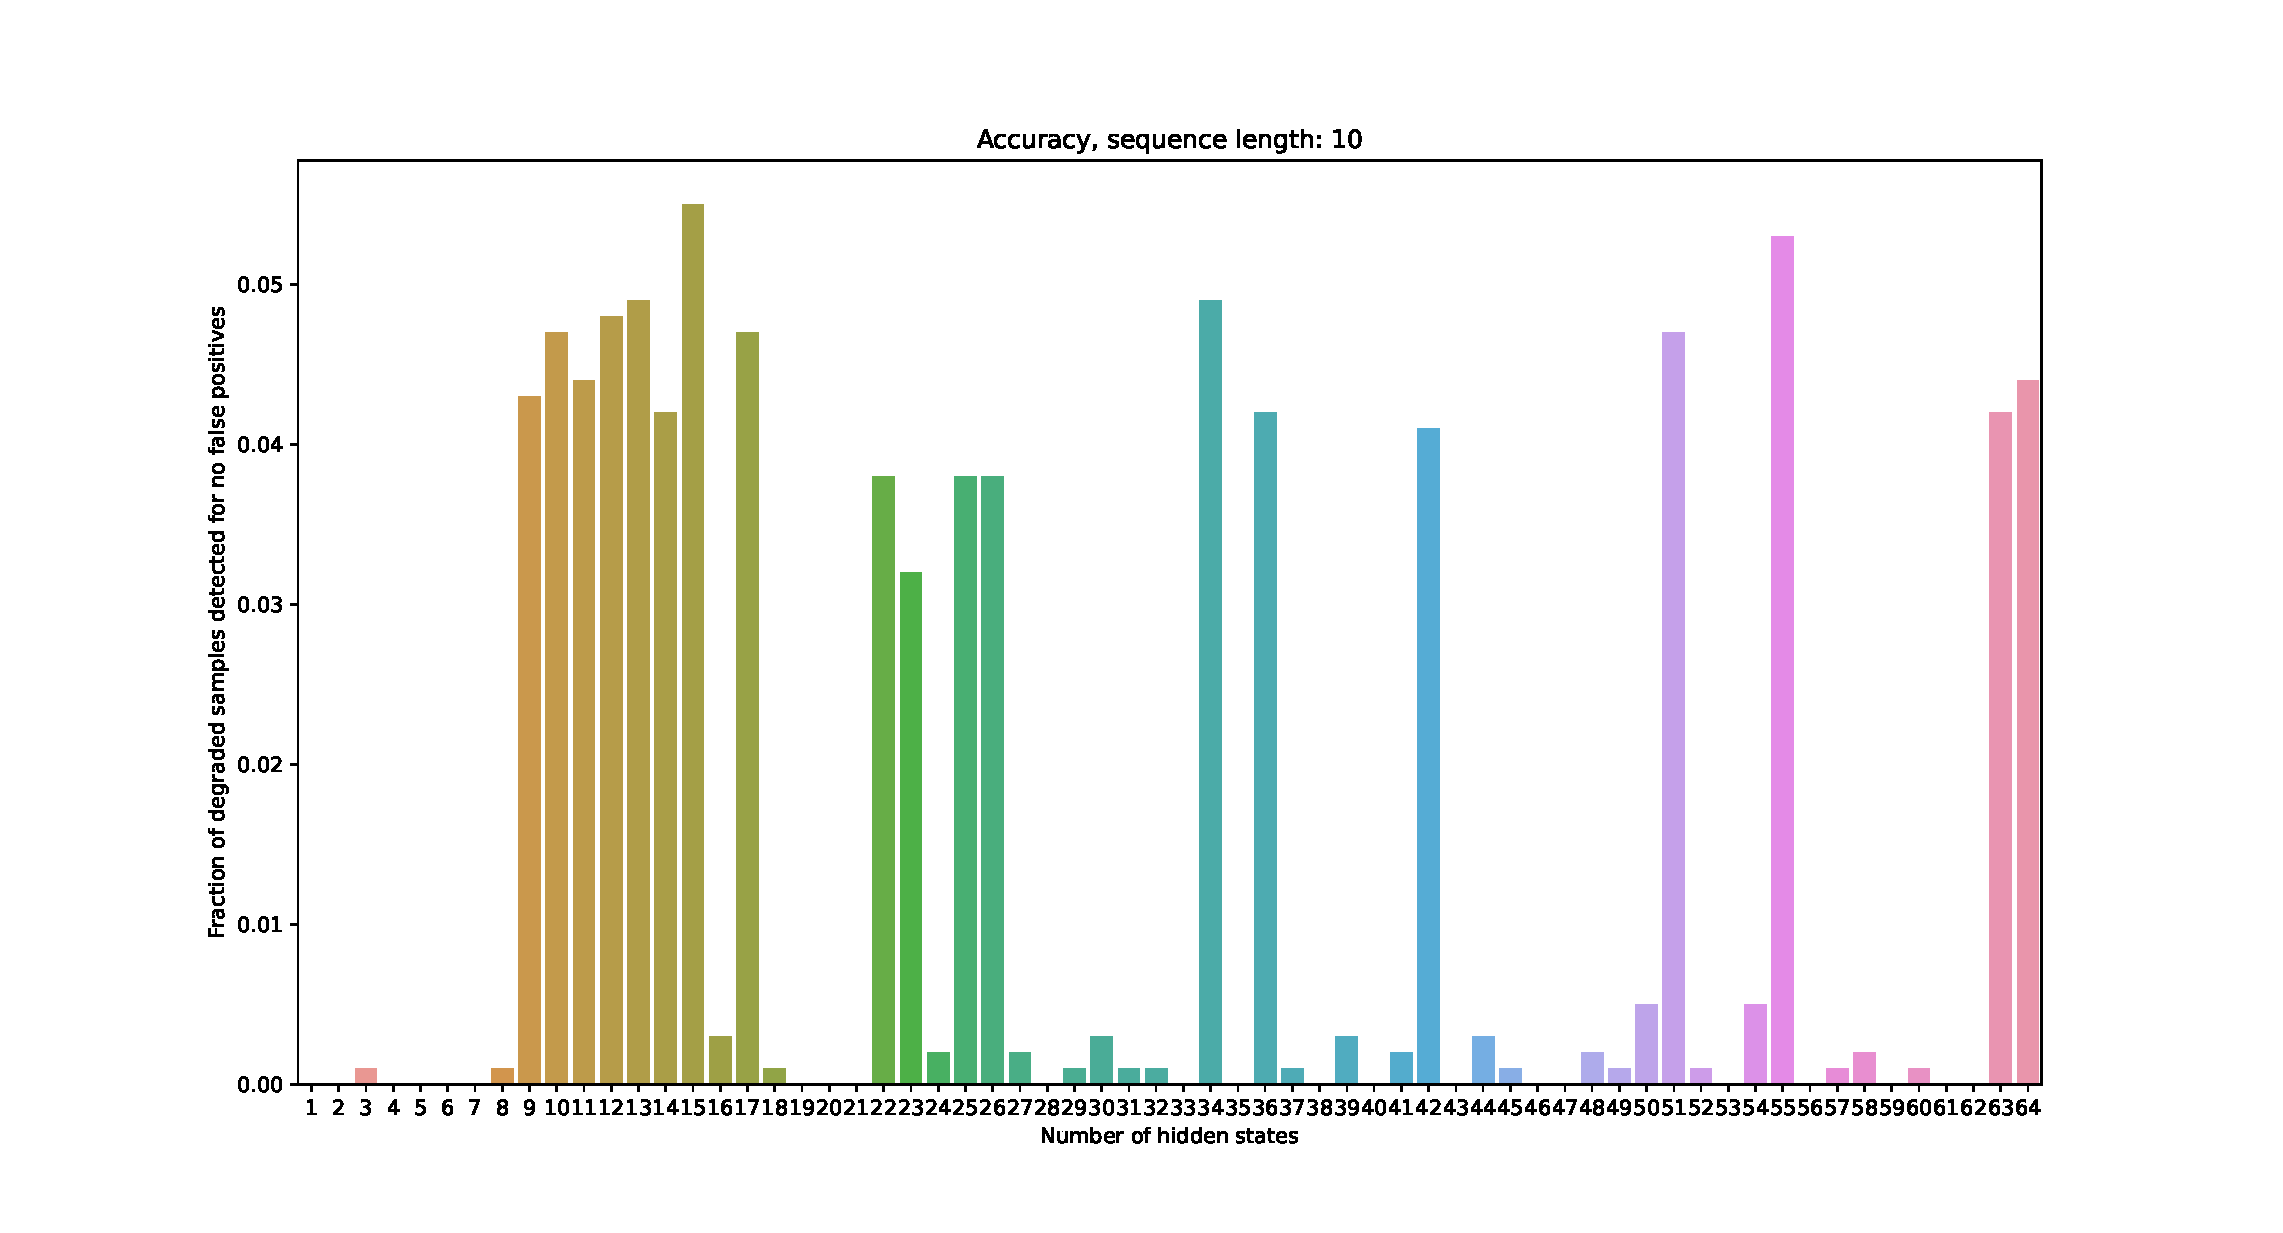
\includegraphics[width=10cm,keepaspectratio=true]{./accuracy_10.eps}
 \caption{KL divergence score based correct discrimination fraction for degraded samples for no false positives with a sequence length of 10.}
 \label{figure:discrimination_rate_10}
\end{figure}

\begin{figure}[h]
 \centering
 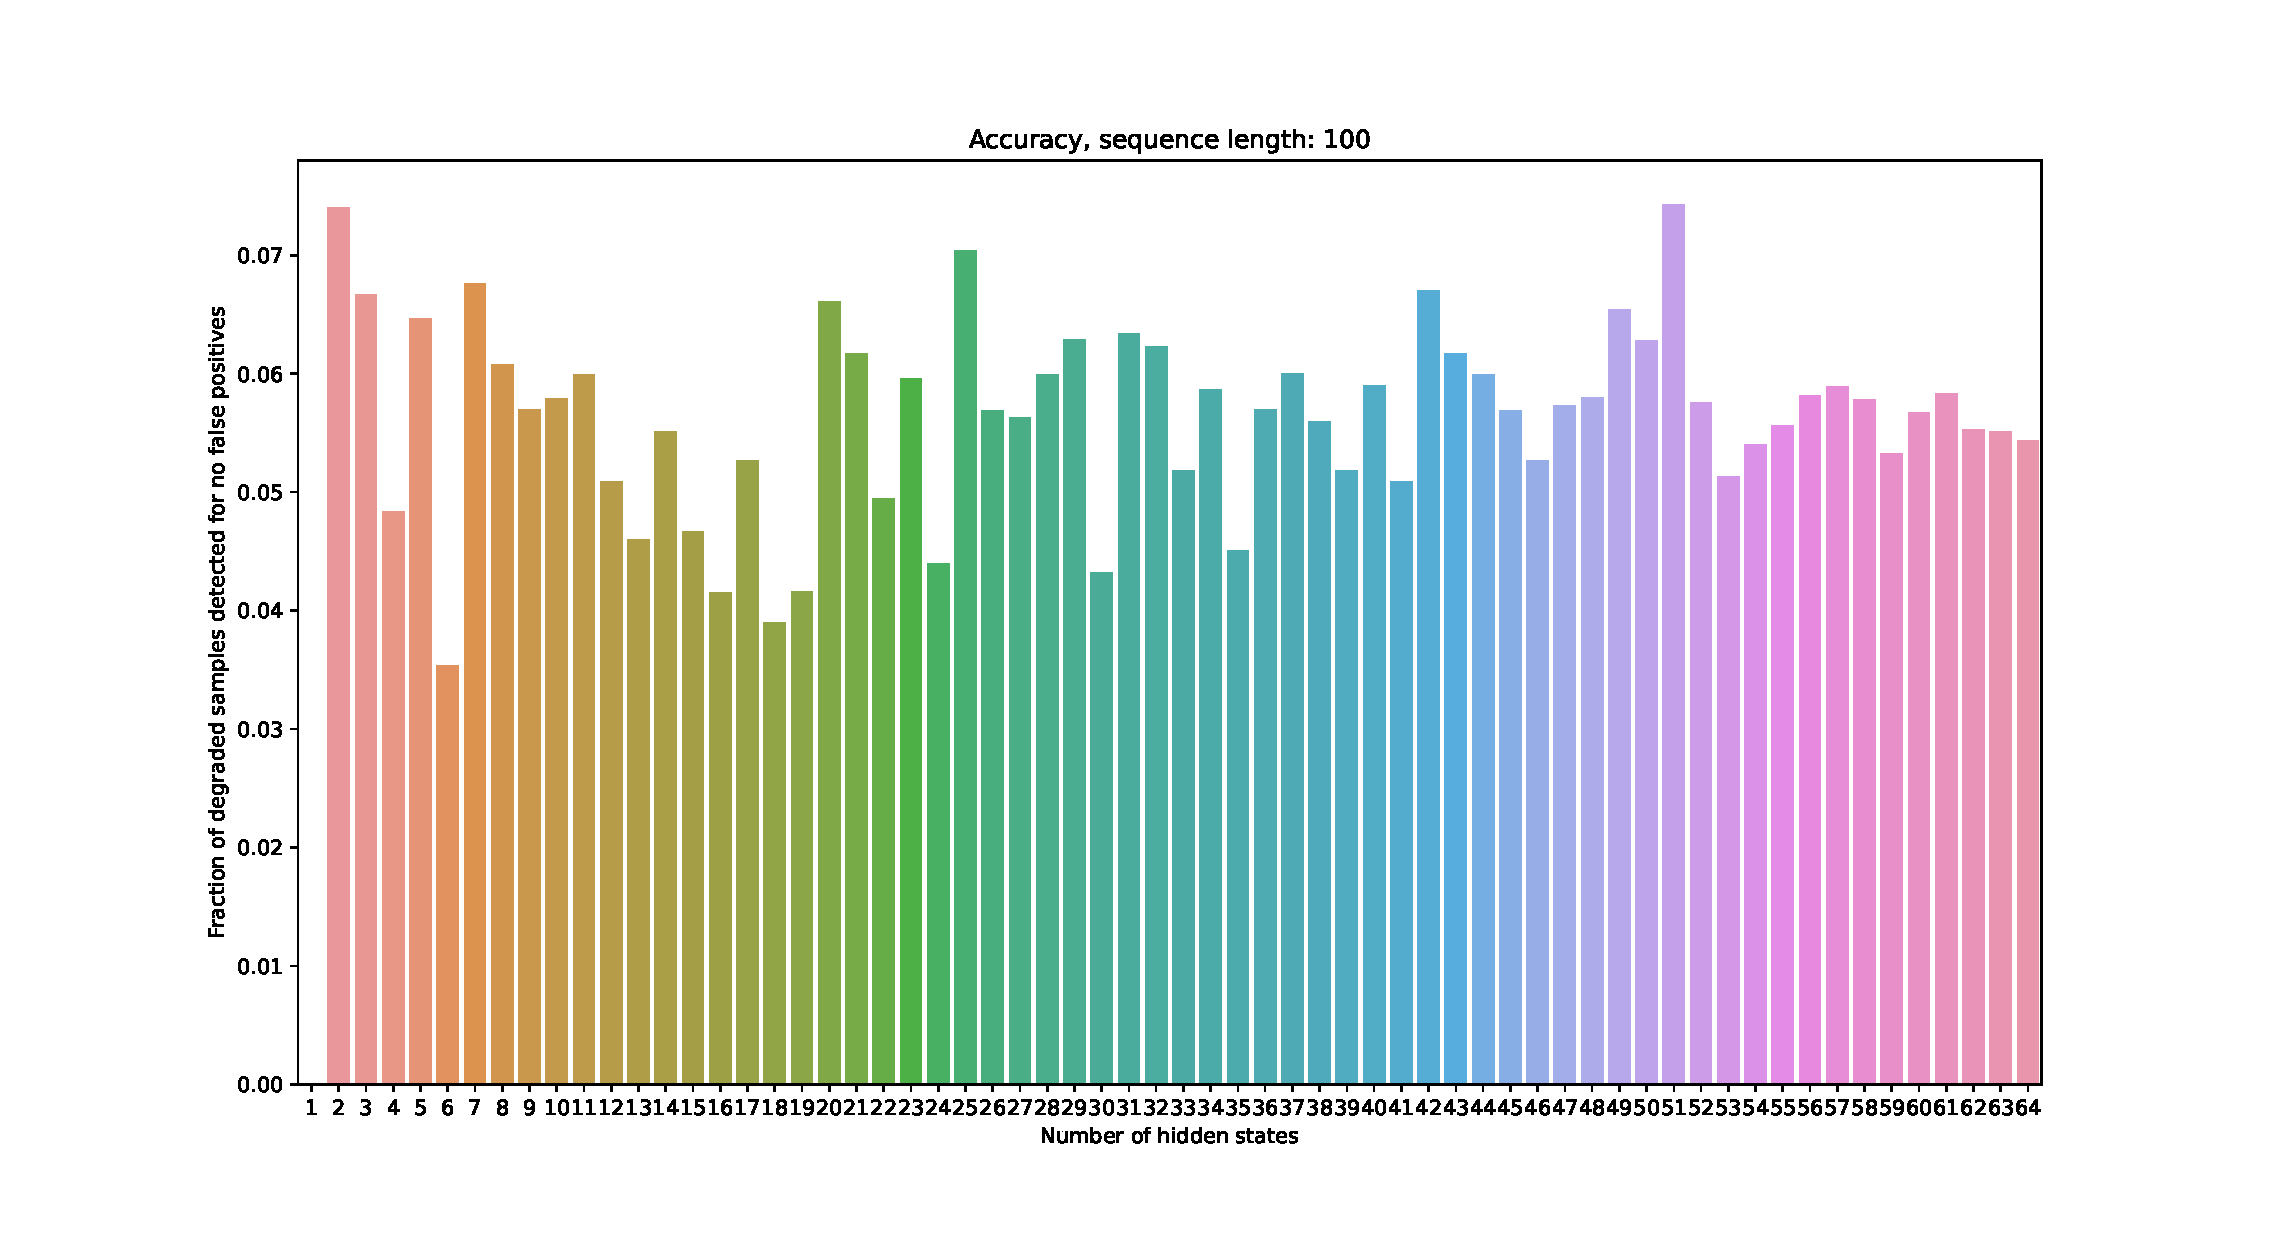
\includegraphics[width=10cm,keepaspectratio=true]{./accuracy_100.eps}
 \caption{KL divergence score based correct discrimination fraction for degraded samples for no false positives with a sequence length of 100.}
 \label{figure:discrimination_rate_100}
\end{figure}

\begin{figure}[h]
 \centering
 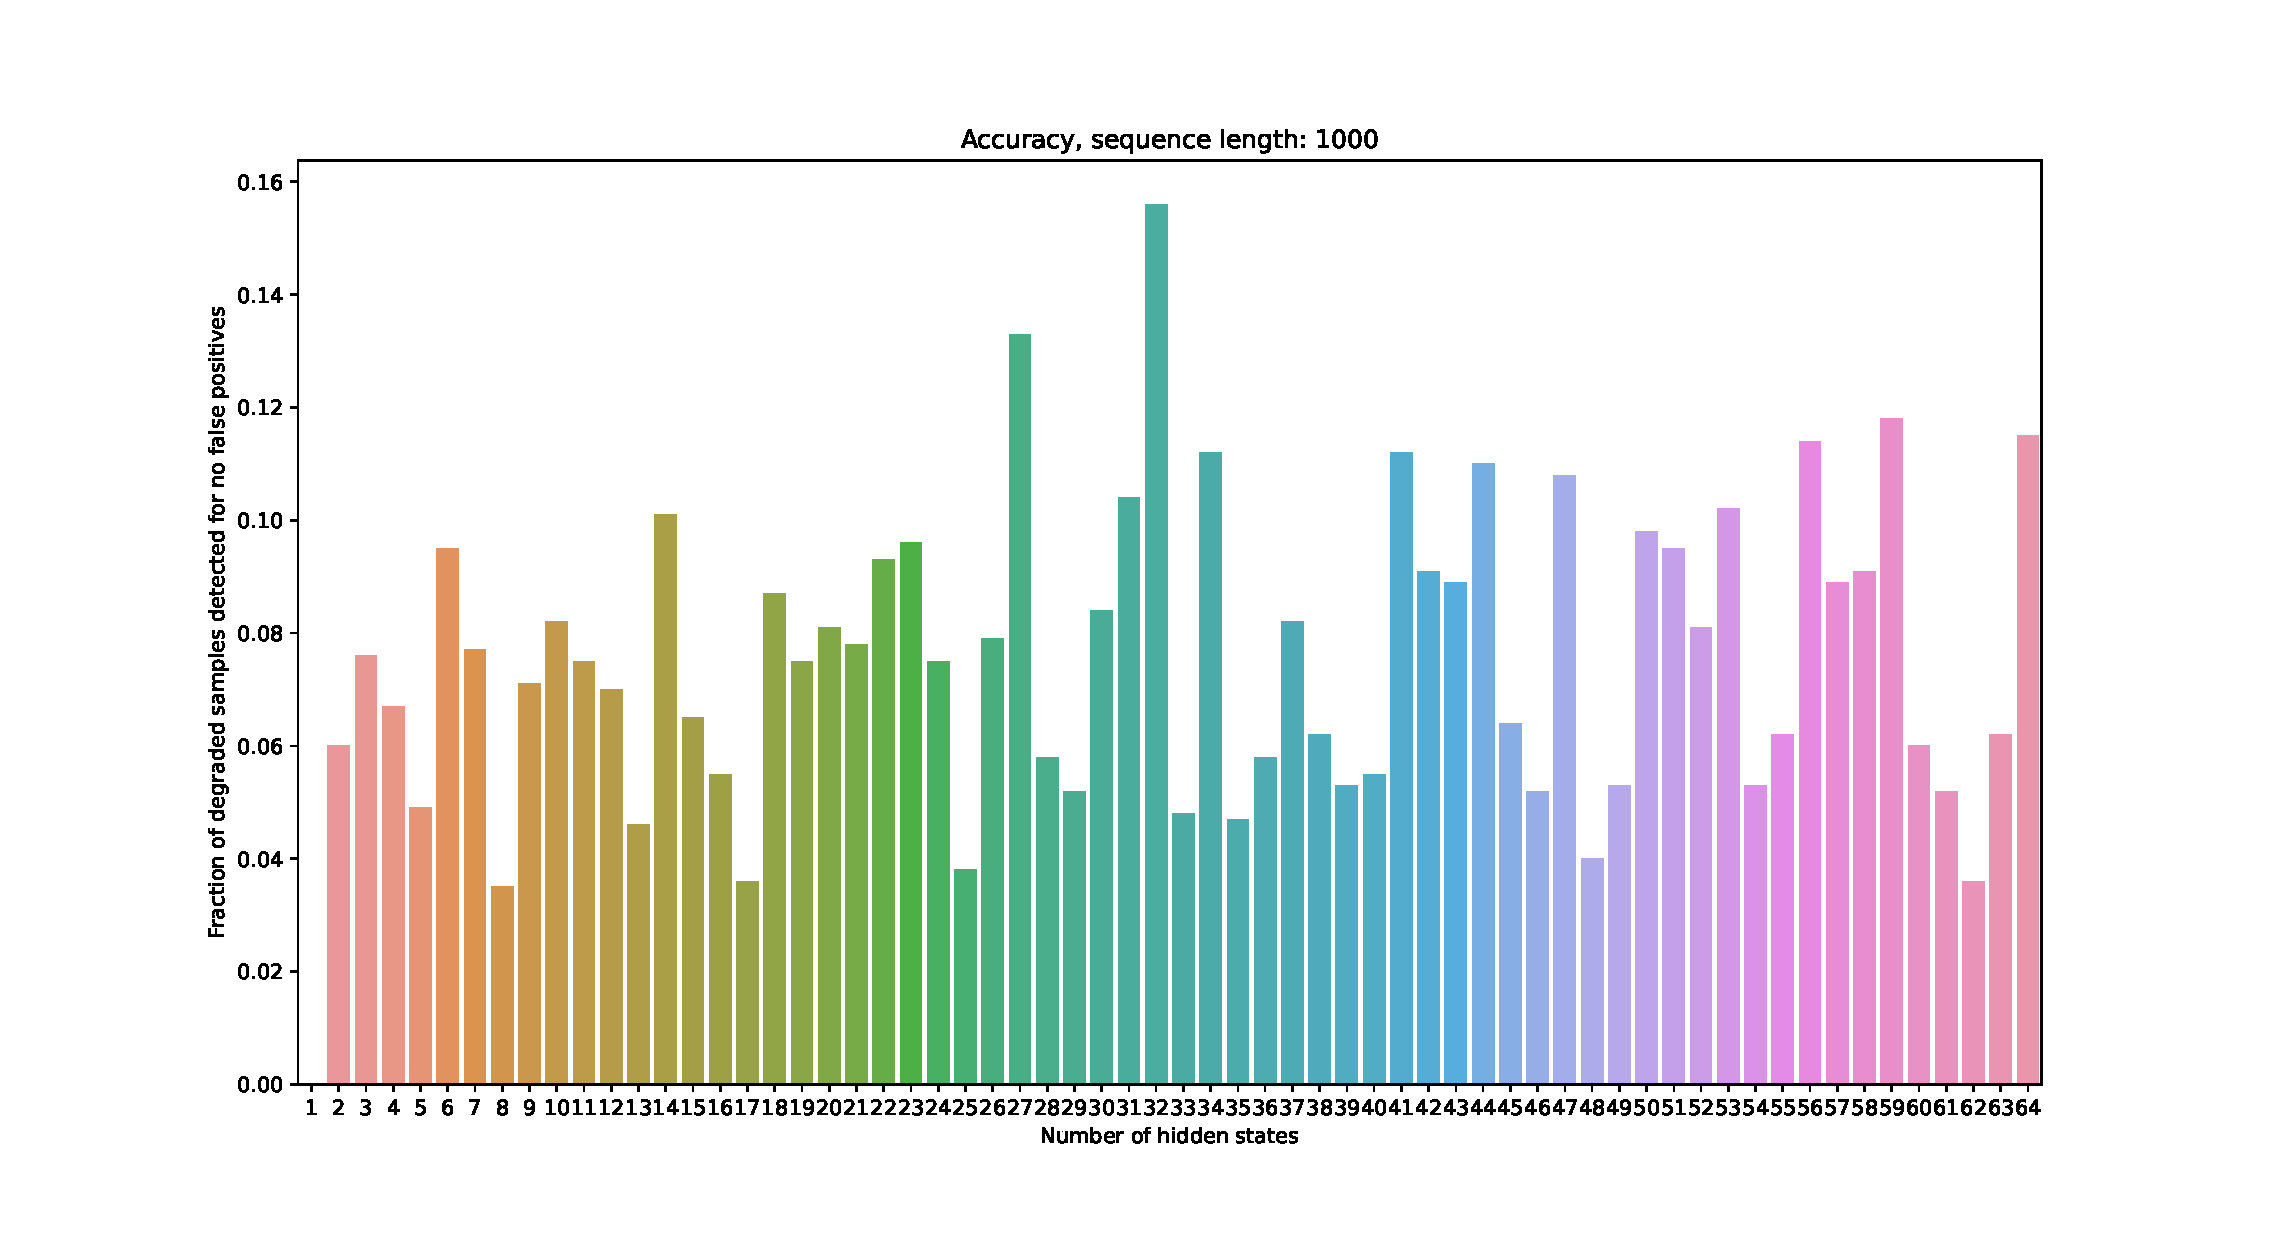
\includegraphics[width=10cm,keepaspectratio=true]{./accuracy_1000.eps}
 \caption{KL divergence score based correct discrimination fraction for degraded samples for no false positives with a sequence length of 1000.}
 \label{figure:discrimination_rate_1000}
\end{figure}


\end{document}
